\documentclass[11pt,a4paper]{article}
\usepackage[T1]{fontenc}
\usepackage[utf8]{inputenc}
\usepackage[margin=2.4cm]{geometry}
\usepackage{amsmath}
\usepackage{booktabs}
\usepackage{graphicx}
\usepackage{caption}
\usepackage{microtype}
\usepackage[hidelinks]{hyperref}
\captionsetup{font=small,labelfont=bf}
\graphicspath{{fig/}}
\newcommand{\degC}{$^{\circ}$C}
\newcommand{\degree}{$^{\circ}$}
\newcommand{\code}[1]{\texttt{#1}}

\title{Freezing of the world ocean by ice-nine\\[4pt]\large A scenario study with a global column model}
\author{Erik Wistrand}
\date{19 October 2026}

\begin{document}
\maketitle

\begin{abstract}
Ice-nine, from Vonnegut's \emph{Cat's Cradle}, is a solid phase of water that melts at 45.8~\degC. We simulate its spread through the world ocean from a single seed with a global grid model that includes latent heat, air-sea exchange, a seasonal atmosphere with water vapour and clouds, and snowfall of ice-nine, in 25 twelve-year scenarios. Latent heat stops the freeze: 39\% of the ocean by mass freezes within a week, seeded far ahead of the front by rain that airborne crystals have frozen, and 44\% after twelve years. The same rain whitens most land within two weeks. Whether ice-nine sinks or floats decides the end. A sinking solid leaves an open slush ocean near 42~\degC\ under air near 35~\degC. A floating solid closes a crust after 5.8 years and cools the air to $-37$~\degC\ after twelve, about 20~K of it through clouds; leads covering 1\% of the crust would leave the air 19~K warmer.
\end{abstract}

\section{Introduction}

\noindent
\begin{minipage}[t]{0.56\textwidth}
\setlength{\parindent}{1.5em}
\noindent In the novel, a crystal of ice-nine falls into the sea and the oceans freeze almost at once. Seawater at 0--30~\degC\ is 15--45~K below the melting point of the new phase, so contact growth is plausible. Freezing, however, releases latent heat, and that heat has to go somewhere. This paper asks how much of the ocean freezes, how fast, what limits it, and what happens to the air and the land. Figure~\ref{fig:timeline} summarises the course of events in both scenarios.

The idea is older than the novel. Vonnegut worked in public relations at General Electric in Schenectady from 1947, where his brother Bernard worked in Irving Langmuir's group on seeding supercooled clouds with dry ice and silver iodide. By Vonnegut's own account, ice-nine was Langmuir's: a laboratory legend had it that Langmuir, assigned to host H.\,G.\ Wells on a visit to Schenectady, offered him the idea of ``a form of ice that was stable at room temperature'' for a story; Wells never used it, and after Wells (1946) and Langmuir (1957) had died, Vonnegut took it (``Finders, keepers''), making Langmuir the model for Felix Hoenikker (Vonnegut, \emph{The Paris Review} 69, 1977). Elsewhere the idea is credited to Bernard Vonnegut (\emph{Physics Today} 39(11), 1986). The melting point of 45.8~\degC\ is the novel's own; we found no source for the number.
\end{minipage}\hfill
\begin{minipage}[t]{0.40\textwidth}
\vspace{0pt}
\centering
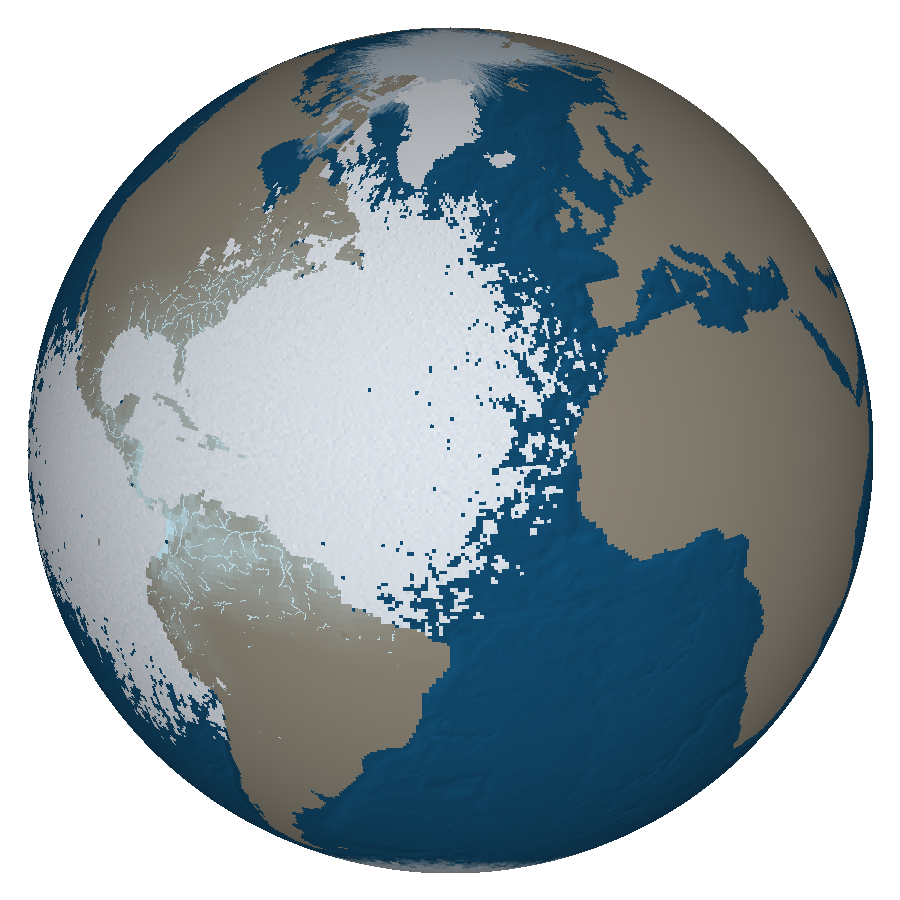
\includegraphics[width=\linewidth]{globe_sinks_48h.png}
\captionof{figure}{Sinking ice-nine two days after a seed in the Caribbean (0.5\degree\ grid, 10-minute steps). Seeded sea is pale grey to white with its solid fraction (0 to 100\%); unseeded sea is blue. Rain carrying crystals has seeded the North Atlantic and the eastern Pacific far ahead of the contact front, which has moved about 700~km; the ocean is 5\% frozen by mass.}
\label{fig:title}
\end{minipage}

\clearpage
\subsection*{Main findings}

\begin{enumerate}
\item \textbf{The ocean stalls at 39\% within a week.} Each column freezes until its own latent heat brings it to the melting point. Further freezing is limited by how fast heat leaves the planet, about 0.4 percentage points per year (Section~\ref{sec:phases}).
\item \textbf{Rain, not the front, freezes the ocean.} Crystals lofted from seeded water freeze the rain they meet, and that rain seeds open water wherever it falls. With 2-hour steps the ocean is 10\% frozen after 3 days and 38\% after 7. Without snowfall the same 39\% takes about 60 days, set by the front speed (Section~\ref{sec:speed}).
\item \textbf{The land turns white within two weeks.} The same rain falls on land as ice-nine snow: 93\% of land is white after 10 days. Fresh ice-nine melts at 45.8~\degC, the sea slush at 43.6~\degC\ or lower, and the air over a slush ocean stays close to the slush, so snow survives everywhere except in continental summers. How much land turns white depends on unconstrained crystal parameters: 5 of 54 tested combinations keep more than 80\% of land white after one year (Section~\ref{sec:snow}).
\item \textbf{The air overshoots.} With 2-hour steps the mean air temperature peaks at 43~\degC\ on day 16, then settles near 36~\degC\ within a month. The polar air warms most: 40~K above climatology at 60--90\degree N against 17~K in the tropics, because polar water starts 44~K below the melting point and tropical water only 17~K (Section~\ref{sec:air}).
\item \textbf{The floating case ends in a deep snowball.} The crust closes after 5.8 years. Brine rejected by the growing crust makes the water below it denser than the deep water, the two overturn, and the deep ocean freezes within about two years instead of waiting for the crust. The air falls below 14~\degC\ after 4.7 years, below 0~\degC\ after 5.6, and reaches $-37$~\degC\ after twelve (Section~\ref{sec:floats}).
\item \textbf{Clouds deepen the snowball by about 20~K.} Under a closed crust evaporation stops, cloud cover falls from 0.80 to 0.28, and the white surface shows through. Without clouds the floating case ends at $-17$~\degC, without the water-vapour greenhouse at $-29$~\degC, without snowfall at $-25$~\degC.
\item \textbf{Leads weaken the snowball.} The floating results assume a sealed crust. Keeping 0.3\% of the crust open as leads warms the air after twelve years by 8~K, 1\% by 19~K: the deep water under the crust is near 42~\degC, and the vapour from the leads keeps the clouds. A plausible open-water equivalent of 0.15--0.9\% puts the end state between about $-33$ and $-20$~\degC\ (Section~\ref{sec:leads}).
\item \textbf{Front speed, currents, bathymetry and the diurnal cycle} change the first weeks but not the twelve-year result.
\end{enumerate}

\clearpage
\begin{figure}[!t]
\centering
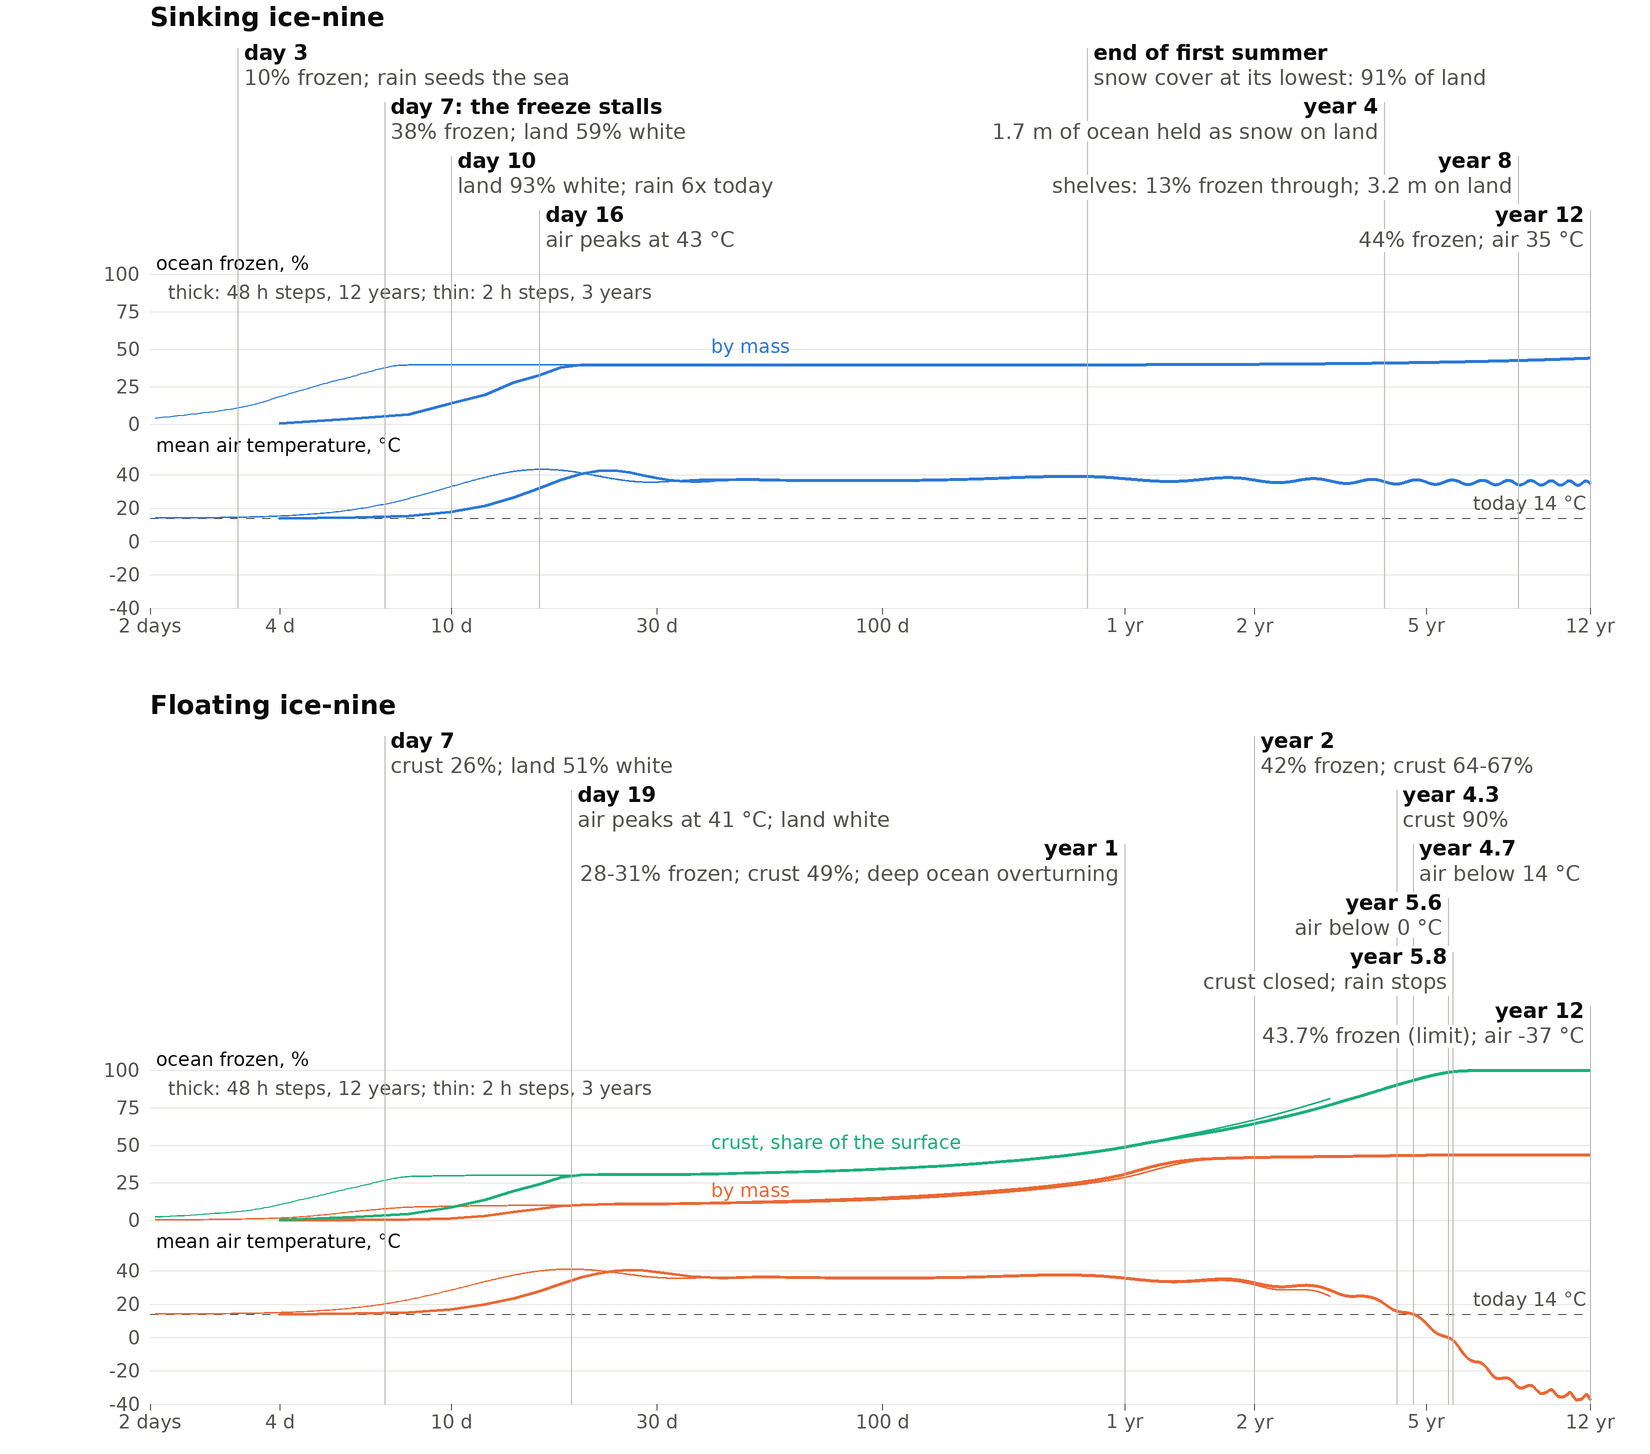
\includegraphics[width=\textwidth]{timeline.png}
\caption{Timeline of the two baseline scenarios (0.5\degree\ grid, single seed in the Caribbean, front speed 15~km/h), on a logarithmic time axis. Each panel shows the ocean frozen (by mass; for the floating case also the share of the surface under crust) and the mean air temperature. Thick lines: the twelve-year runs with 48-hour steps. Thin lines: three-year runs with 2-hour steps, which resolve the first weeks (Section~\ref{sec:conv}). Events up to year 3 are taken from the 2-hour runs, later ones from the 48-hour runs. The yearly oscillation in air temperature is the seasonal cycle.}
\label{fig:timeline}
\end{figure}

\section{Model}
\label{sec:model}

\subsection{Grid and processes}

The ocean is represented as columns on a 0.5\degree\ grid derived from the NOAA GLOBE 1~km land mask and Natural Earth bathymetry. Each column has a depth, a temperature $T$ and a solid fraction $\phi$. The atmosphere is a 1\degree\ grid of air columns. Statistics are weighted by cell area. Table~\ref{tab:model} lists the processes.

\begin{table}[htbp]
\centering\small
\caption{Model processes.}
\label{tab:model}
\begin{tabular}{p{3.0cm}p{11.8cm}}
\toprule
Process & Representation \\
\midrule
Front & A seeded column seeds its neighbours at a prescribed speed (default 15~km/h), isotropic in kilometres. \\
Freezing & A seeded column freezes while below its melting point and melts back when above it. The melting point falls as brine concentrates, by $2.2/(1-\phi)$~K, capped at 16~K where NaCl saturates. Latent heat stays in the freezing column. Solid ice-nine has half the heat capacity of water, and the latent heat varies with temperature accordingly (Kirchhoff), so freezing and melting conserve enthalpy exactly. \\
Air-sea exchange & Bulk sensible, latent and longwave fluxes against climatology: a stratified column's own mean, today's sea surface once the lattice has mixed it. The turbulent part warms the air. Evaporation comes only from the unfrozen share of the surface. \\
Atmosphere & Air temperature with an annual and seasonal climatology by latitude and land share. The anomaly is carried by large-scale eddy mixing ($10^6$~m$^2$/s) and zonal winds up to 8~m/s. Each cell radiates with a Planck response weakened by a water-vapour greenhouse and the cloud feedback. A white surface (floating crust, a sinking column frozen through, snow on land) reflects sunlight; clouds hide part of it. The air's warming may exceed the sea surface's warming at its latitude by at most 3~K (moist convection); the excess is spread over the whole atmosphere, so energy is kept. \\
Water cycle & A vapour field fed by evaporation and carried with the air sets rain over land (today's map, from the GPCC climatology for 1971--2000 (Rustemeier et al.\ 2025, Deutscher Wetterdienst), with 171~mm/yr over Antarctica (Palerme et al.\ 2014), plus the extra vapour) and cloud cover. The latent heat of the extra evaporation travels with the vapour and warms the air where it rains out. \\
Snowfall & Sea spray lofts crystals from seeded water; they travel with the air and are washed out by rain. Rain falling through air carrying crystals, below 45.8~\degC, lands as ice-nine: as snow on land, and as seed on lakes, rivers and the open sea. Snow melts where the air or sunlit ground is above the melting point. \\
Currents & Prescribed gyres and zonal currents exchange heat between neighbouring columns (heat-conserving) and carry crystals downstream; flow weakens under ice. \\
Other & Diurnal and seasonal insolation, seasonal sea ice, Greenland and Antarctic ice sheets, airborne seeding by storms (used only when snowfall is off, since rain seeding replaces it). Optional: algae in the brine of a floating crust (Section~\ref{sec:life}). \\
\bottomrule
\end{tabular}
\end{table}

\subsection{Sinking and floating solid}
\label{sec:columns}

The novel does not state whether ice-nine is denser than water. The answer determines the vertical structure, and we model both cases (Figure~\ref{fig:columns}).

\paragraph{Sinking solid.} Crystals sink through supercooled water and grow as they fall, so a column becomes a slush over its full depth within hours. A single temperature per column is used. This is the default.

\paragraph{Floating solid.} A crust forms at the surface and the latent heat warms the water directly below it. Each column is split into a 100~m mixed layer, which interacts with the front and the air, and a deep layer with its own temperature and salinity. The layers exchange heat by eddy diffusion ($10^{-4}$~m$^2$/s) through liquid or by conduction ($10^{-6}$~m$^2$/s) through the crust. The crust rejects salt. When the mixed layer's liquid is denser than the deep liquid (UNESCO equation of state), the two overturn at 0.02~m/s, a typical open-ocean convective velocity, mixing heat and salt; the deep water then freezes against the crystals it meets.

Known ice phases other than ordinary ice are denser than water; the real ice~IX has a density of 1.16~g/cm$^3$. This favours the sinking case. The cold, ice-covered world at the end of the novel corresponds to the floating case. The floating crust is sealed by default; Section~\ref{sec:leads} tests a crust with leads.

\begin{figure}[htbp]
\centering
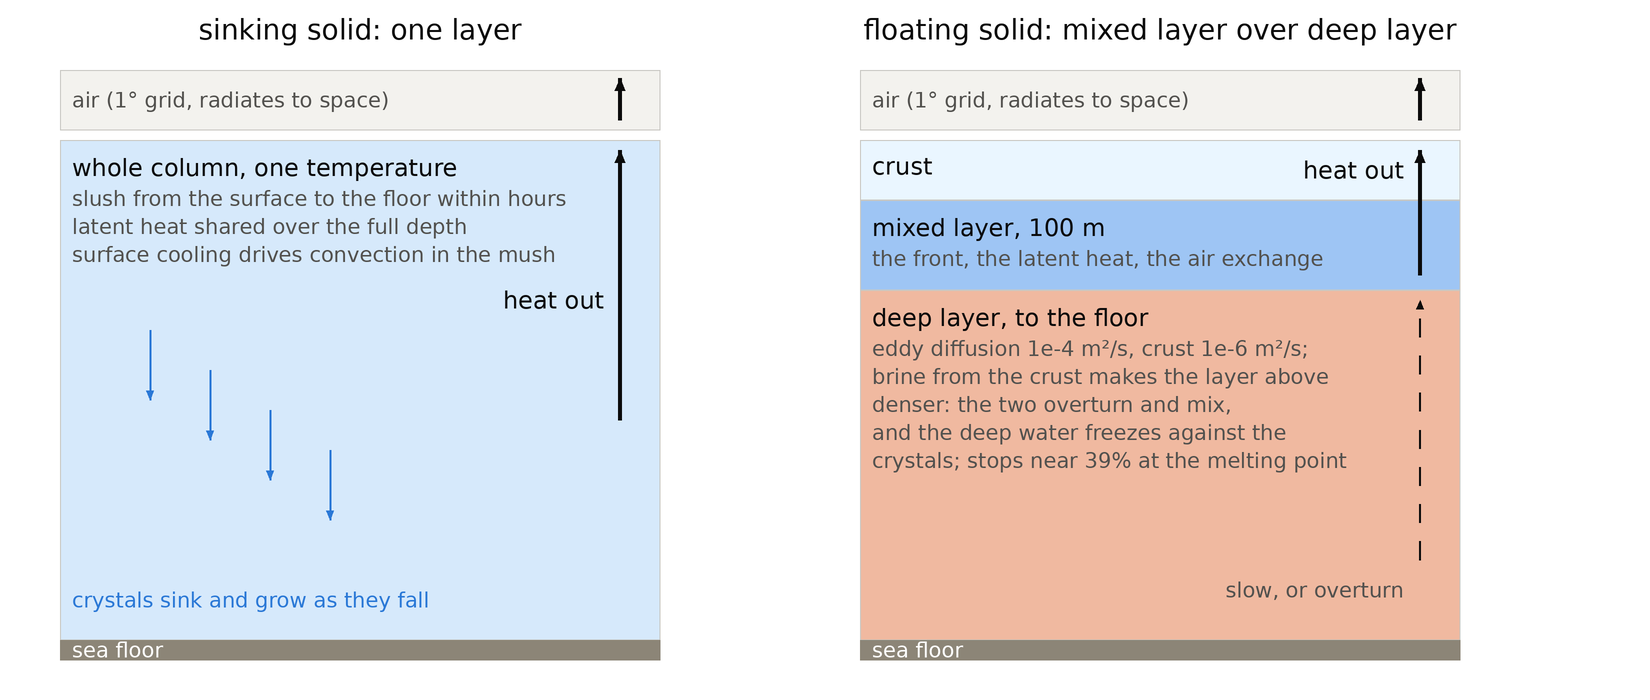
\includegraphics[width=\textwidth]{columns.png}
\caption{The two column models. Left: single layer (sinking solid). Right: mixed layer over a deep layer (floating solid).}
\label{fig:columns}
\end{figure}

\section{Physical constants}
\label{sec:const}

Table~\ref{tab:const} lists the main constants and their sources. Where the model has a user control, the control scales the value in the table.

\begin{table}[htbp]
\centering\small
\caption{Physical constants. Bulk coefficients assume a 7~m/s wind. Values marked $\sim$ are approximate climatology or estimates.}
\label{tab:const}
\begin{tabular}{p{4.2cm}p{3.6cm}p{6.8cm}}
\toprule
Quantity & Value & Basis \\
\midrule
Latent heat of fusion & 389 kJ/kg at the melting point & Entropy of fusion of known ice phases, 20--22 J/mol/K, at 319 K \\
Melting-point depression & 2.2 K, as $1/(1-\phi)$, max 16 K & Cryoscopic constant at 319 K; brine concentration; NaCl saturation \\
Sensible heat flux & 10 W/m$^2$/K & Bulk formula \\
Latent heat flux & 22 W/m$^2$/K at 20~\degC, doubling per 12 K & Bulk formula with Clausius-Clapeyron \\
Net longwave (sea) & 5 W/m$^2$/K & Linearised surface emission \\
Planck response & 3.3 W/m$^2$/K at 288 K & 35-day relaxation of a $10^7$~J/m$^2$/K air column \\
Water-vapour feedback & 1.3 W/m$^2$/K today, growing to cancel the Planck response near 330 K & IPCC AR6 (with lapse rate); runaway threshold \\
Cloud feedback & 0.42 W/m$^2$/K & IPCC AR6 central estimate \\
Cloud masking & cover 0.67 today, up to 0.9; 30\% transmission & Halves the effect of surface albedo at today's cover \\
White ocean & 102 W/m$^2$ & Planetary albedo 0.3 to 0.6 \\
White land & 0.74 of white ocean per m$^2$ & Surface albedo gain 0.55 against 0.74 \\
Air transport & $10^6$~m$^2$/s, 8~m/s & Large-scale eddy diffusivity, low-level winds \\
Convective cap & 3 K & $\sim$ tropical land-over-sea excess today \\
Vapour residence & 9 days & 25 mm precipitable water, 2.7 mm/day rain \\
Overturn velocity & 0.02 m/s & $\sim$ open-ocean deep convection \\
Seasonal air range & 1--17 K by latitude & $\sim$ observed land and sea climatology \\
Crystal lofting, washout, threshold & 24 h, 7 days, $10^{-4}$ & $\sim$ estimates; varied in Section~\ref{sec:snowsens} \\
Snow masking depth & 2 cm water & $\sim$ snow masking depth \\
Lateral heat diffusion (sea) & negligible & Eddy diffusivity $10^3$ m$^2$/s \\
\bottomrule
\end{tabular}
\end{table}

Not derived from first principles: the front speed, the storm seeding rate, the current amplitudes, the basal conditions of the ice sheets, the shape of cloud cover against vapour, the three crystal parameters, and the warming of sunlit ground under snow. The model has no ocean circulation beyond the prescribed surface currents.

For a column that freezes without losing heat, freezing stops when the column reaches its melting point. With initial temperature $T_0$, latent heat $l$ expressed as warming of water per unit solid fraction (93~K), melting point $T_m(\phi)$ and pure melting point $T_{m0}=45.8$~\degC, enthalpy conservation with the solid's half heat capacity gives the final solid fraction $\phi^\ast$ from
\begin{equation}
\left(1-\tfrac{\phi^\ast}{2}\right)T_m(\phi^\ast) - \phi^\ast\left(l-\tfrac{T_{m0}}{2}\right) = T_0 .
\label{eq:stall}
\end{equation}
Deep water at 2--5~\degC\ gives 41--44\%, water at 28~\degC\ only 17\%, polar water at $-1$~\degC\ 47\%. The column ends at about 42~\degC\ in every case.

\section{Scenarios}
\label{sec:scen}

Each scenario runs for twelve simulated years on the 0.5\degree\ grid with a single seed in the Caribbean, in 48-hour steps. The baseline uses the values in Table~\ref{tab:const} and the sinking-solid column. Each other scenario changes one setting. Results are in Table~\ref{tab:scen} and Figure~\ref{fig:f12}. The 48-hour step delays the events of the first weeks by one to two weeks (Section~\ref{sec:conv}); it does not change any value from day 30 on.

\begin{table}[htbp]
\centering\footnotesize
\caption{Scenario results (48-hour steps). Ocean frozen by mass (\%) after 120 days and 1, 5 and 12 years; day on which 99\% of the ocean surface is ice-covered; maximum rise in mean air temperature (K) and the year it occurs; mean air temperature at 12 years (\degC); heat delivered from the sea to the air over twelve years, relative to the sinking baseline; land white with ice-nine snow after one year (\%). ``Radiative response'' scales the Planck, water-vapour, cloud and albedo terms together.}
\label{tab:scen}
\setlength{\tabcolsep}{3pt}
\begin{tabular}{lrrrrrrrrrr}
\toprule
Scenario & 120 d & 1 yr & 5 yr & 12 yr & Covered & Max rise & Year & Air 12 yr & Heat & White 1 yr \\
\midrule
Baseline (sinking) & 39 & 40 & 41 & 44 & -- & 28.5 & 0.1 & 34.9 & 1.00 & 96 \\
No latent heat & 100 & 100 & 100 & 100 & 60 & 0.0 & -- & 14.0 & 0.00 & 0 \\
Front 5 km/h & 39 & 40 & 41 & 44 & -- & 28.0 & 0.1 & 34.9 & 1.00 & 96 \\
Front 41 km/h & 39 & 40 & 41 & 44 & -- & 29.0 & 0.1 & 34.9 & 1.00 & 96 \\
Radiative response 0.25$\times$ & 39 & 40 & 41 & 43 & -- & 29.3 & 0.1 & 35.9 & 0.47 & 82 \\
Radiative response 2$\times$ & 39 & 40 & 42 & 46 & -- & 27.6 & 0.1 & 33.7 & 1.68 & 100 \\
Latent heat 334 kJ/kg & 46 & 46 & 48 & 51 & -- & 27.9 & 0.1 & 34.0 & 1.00 & 98 \\
Latent heat 669 kJ/kg & 23 & 23 & 24 & 26 & -- & 29.8 & 0.1 & 37.0 & 0.92 & 97 \\
No atmosphere & 40 & 44 & 59 & 76 & -- & 0.0 & -- & 14.0 & 0.00 & 0 \\
No diurnal or seasonal cycle & 39 & 40 & 41 & 44 & -- & 29.1 & 0.1 & 35.0 & 0.99 & 99 \\
No currents or storm seeding & 39 & 40 & 41 & 44 & -- & 28.5 & 0.1 & 34.8 & 1.00 & 96 \\
Uniform depth & 39 & 40 & 41 & 43 & -- & 28.5 & 0.1 & 37.8 & 1.03 & 95 \\
No snowfall & 39 & 40 & 41 & 43 & -- & 25.4 & 0.8 & 35.3 & 0.71 & 0 \\
Convective cap 1.5 K & 39 & 40 & 41 & 44 & -- & 28.7 & 0.1 & 34.8 & 1.02 & 97 \\
Convective cap 5 K & 39 & 40 & 41 & 44 & -- & 28.1 & 0.1 & 35.0 & 0.98 & 94 \\
No water-vapour greenhouse & 39 & 40 & 42 & 45 & -- & 27.4 & 0.1 & 34.2 & 1.44 & 100 \\
No clouds & 39 & 40 & 41 & 44 & -- & 28.1 & 0.1 & 34.6 & 1.17 & 99 \\
\midrule
Floating: baseline & 16 & 31 & 43 & 44 & 2108 & 26.5 & 0.1 & $-37.1$ & 1.51 & 100 \\
Floating: front 5 km/h & 16 & 31 & 43 & 44 & 2108 & 26.2 & 0.1 & $-37.1$ & 1.51 & 100 \\
Floating: front 41 km/h & 16 & 31 & 43 & 44 & 2106 & 26.8 & 0.1 & $-37.2$ & 1.51 & 100 \\
Floating: no latent heat & 100 & 100 & 100 & 100 & 60 & 0.0 & -- & 14.0 & 0.00 & 0 \\
Floating: no snowfall & 15 & 28 & 43 & 44 & 2375 & 24.1 & 0.7 & $-25.5$ & 1.17 & 0 \\
Floating: no greenhouse & 17 & 37 & 43 & 44 & 1911 & 25.2 & 0.1 & $-29.4$ & 1.47 & 100 \\
Floating: no clouds & 17 & 34 & 43 & 44 & 2080 & 25.8 & 0.1 & $-16.6$ & 1.14 & 100 \\
Floating: life in the brine & 16 & 30 & 43 & 44 & 2182 & 26.5 & 0.1 & $-37.0$ & 1.47 & 100 \\
\bottomrule
\end{tabular}
\end{table}

\begin{figure}[htbp]
\centering
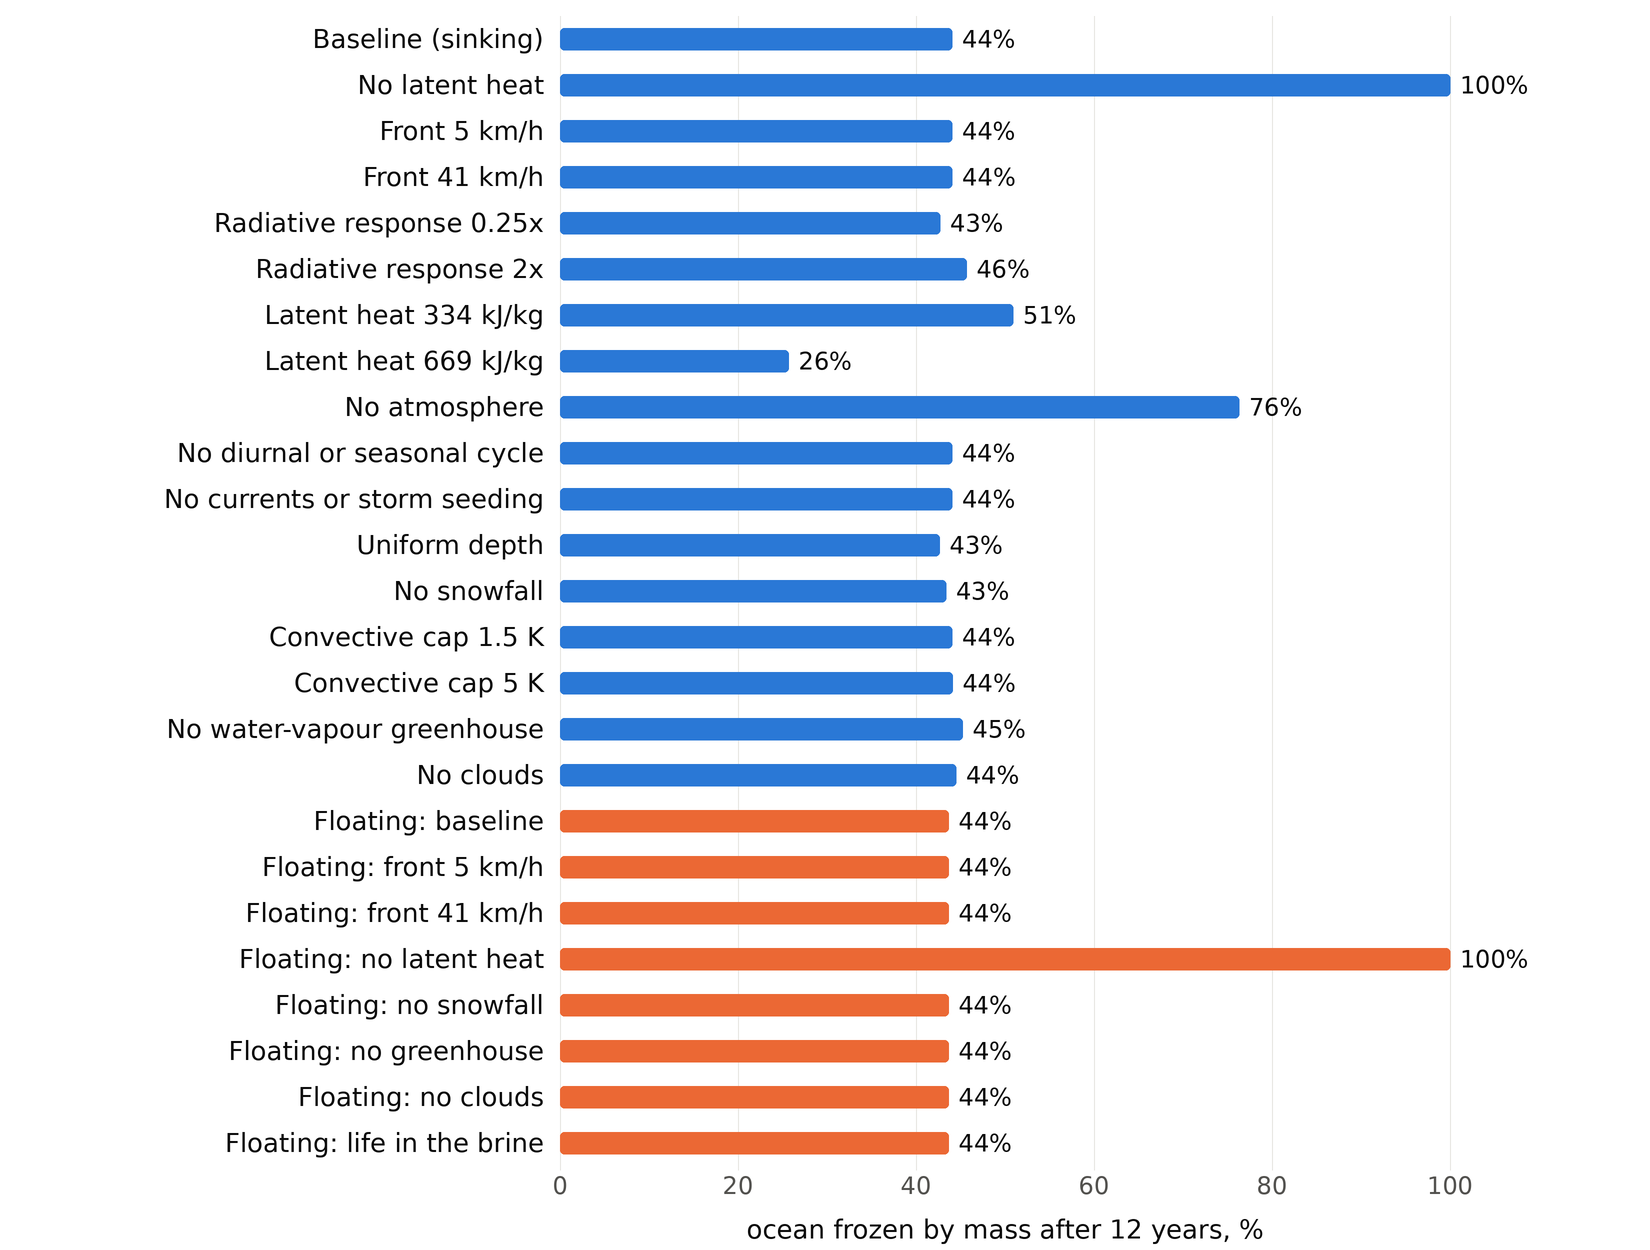
\includegraphics[width=\textwidth]{f12.png}
\caption{Ocean frozen by mass after twelve years.}
\label{fig:f12}
\end{figure}

\subsection{Two phases of freezing}
\label{sec:phases}

In all scenarios with latent heat, freezing has two phases. In the first, each seeded column freezes until its own latent heat brings it to the melting point: 39.4\% of the ocean by mass, reached after 7 days with 2-hour steps. In the second, columns freeze only as fast as heat leaves through the surface and the atmosphere radiates it to space: 0.4 percentage points per year in the sinking baseline, 44\% after twelve years. At that rate the remaining ocean would take about 140 years to freeze.

Without latent heat the ocean freezes completely in 60 days (Figure~\ref{fig:vonnegut}). This is the only scenario in which it does. Without an atmosphere, heat leaves the sea directly and the ocean reaches 76\% after twelve years.

\begin{figure}[htbp]
\centering
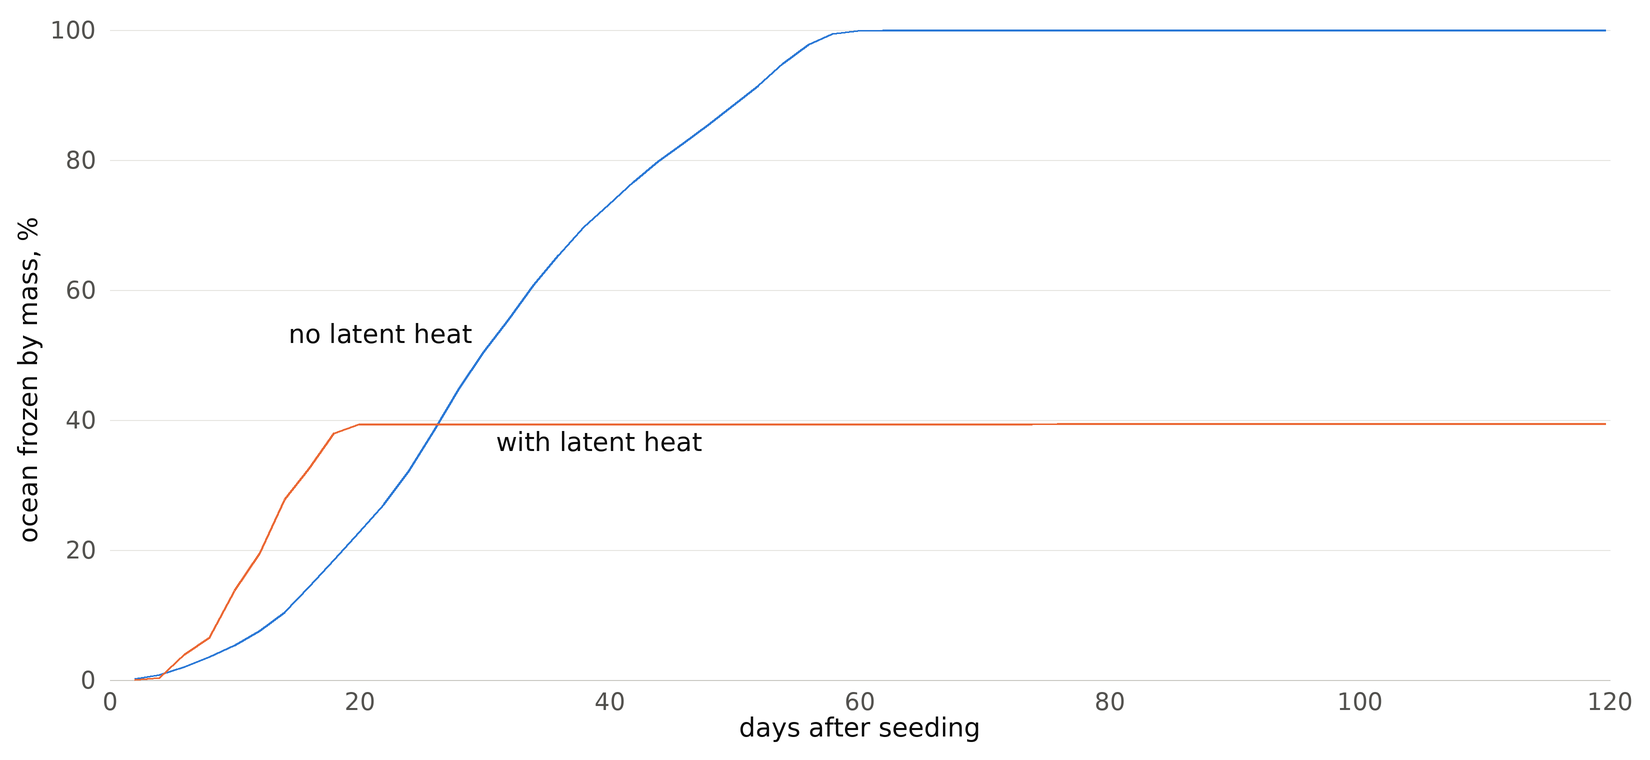
\includegraphics[width=\textwidth]{vonnegut_frozen.png}
\caption{Ocean frozen by mass in the first 120 days, with and without latent heat (48-hour steps).}
\label{fig:vonnegut}
\end{figure}

\subsection{Rain seeding and front speed}
\label{sec:speed}

Rain carrying crystals seeds every patch of open water it falls on, so the ocean is seeded from the sky at thousands of points instead of from one growing front. With 2-hour steps the sinking ocean is 10\% frozen after 3 days and 38\% after 7; rain over land peaks at 6.4 times today's on day 10, driven by evaporation from the warming slush. Without snowfall, which also turns off rain seeding, the front alone takes about 60 days to reach the same 39\% (8.0\% after 20 days against 39.4\% with snowfall, both at 48-hour steps).

Front speed matters only through this race. At 41, 15 and 5~km/h the first phase ends after about 15, 20 and 25 days with 48-hour steps (Figure~\ref{fig:speed}); with 2-hour steps rain seeding finishes it in a week at 15~km/h. After the first month the runs agree to within 0.1 percentage points.

\begin{figure}[htbp]
\centering
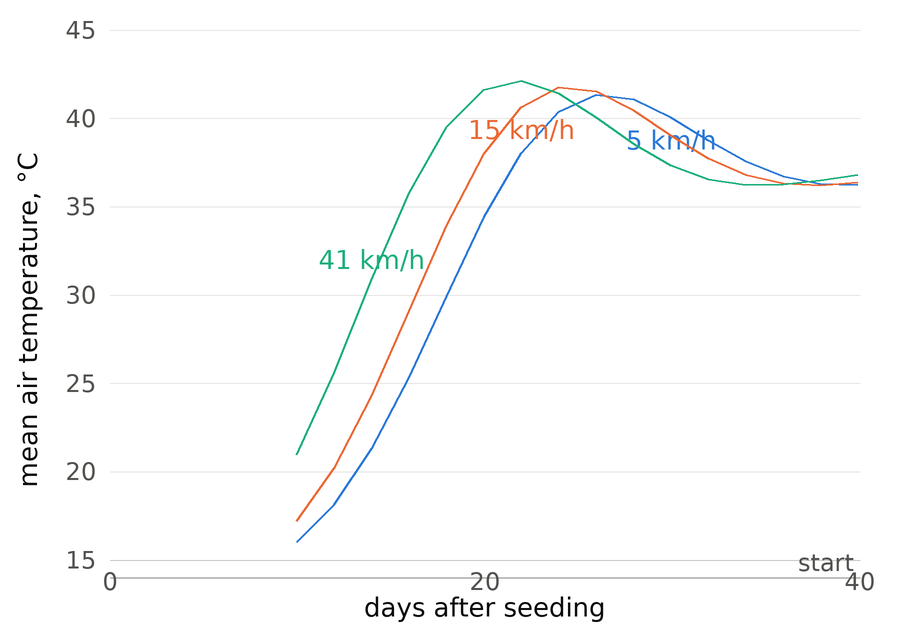
\includegraphics[width=0.49\textwidth]{speed_air.png}
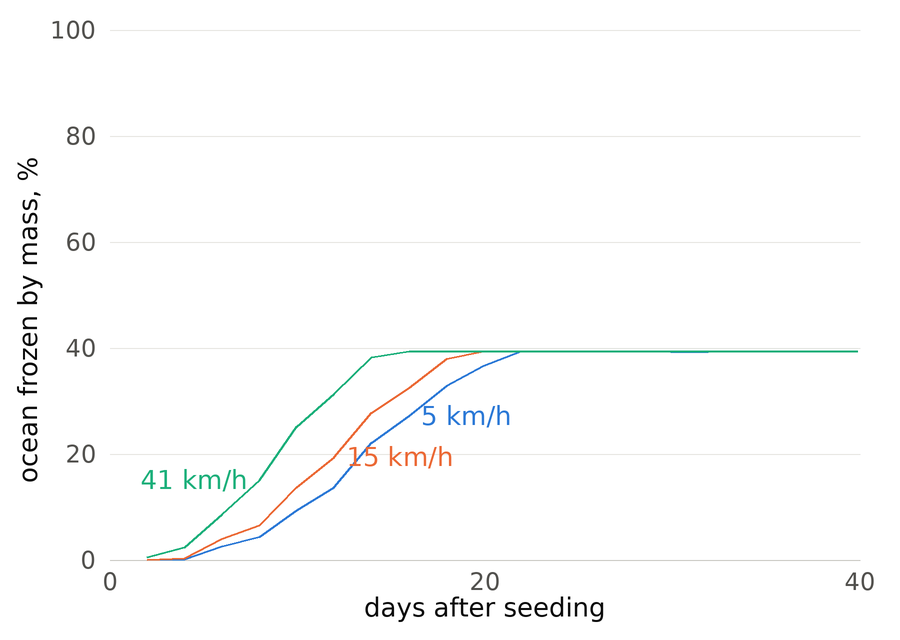
\includegraphics[width=0.49\textwidth]{speed_frozen.png}
\caption{Front speed, first 40 days (48-hour steps). Left: mean air temperature. Right: ocean frozen by mass.}
\label{fig:speed}
\end{figure}

\subsection{Latent heat}

The latent heat determines the fraction frozen in the first phase: 46\% at 334~kJ/kg, 39\% at 389~kJ/kg and 23\% at 669~kJ/kg (Figure~\ref{fig:latent}). The rate in the second phase is about the same in all three.

\begin{figure}[htbp]
\centering
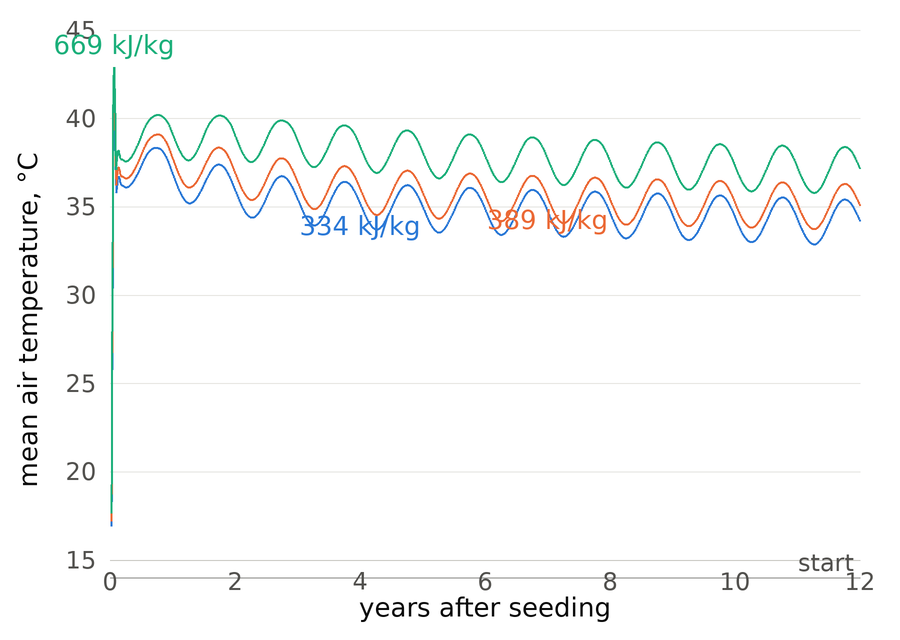
\includegraphics[width=0.49\textwidth]{latent_air.png}
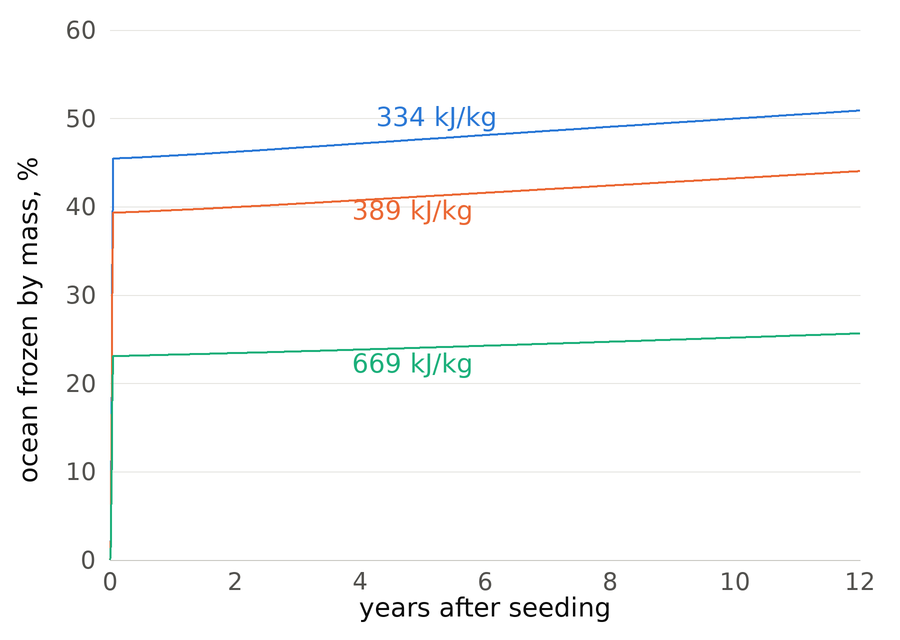
\includegraphics[width=0.49\textwidth]{latent_frozen.png}
\caption{Latent heat. Left: mean air temperature. Right: ocean frozen by mass.}
\label{fig:latent}
\end{figure}

\subsection{Radiation to space}

The second phase depends on how fast the atmosphere loses heat to space. Scaling the radiative response by 0.25 gives 43\% at twelve years with the air at 36~\degC; scaling it by 2 gives 46\% with the air at 34~\degC\ (Figure~\ref{fig:cool}). Removing the water-vapour greenhouse gives 45\% and air 0.7~K cooler; removing clouds changes neither by more than half a unit. The effect on air temperature is small because the air is tied to the sea surface, which sits at the melting point.

\begin{figure}[htbp]
\centering
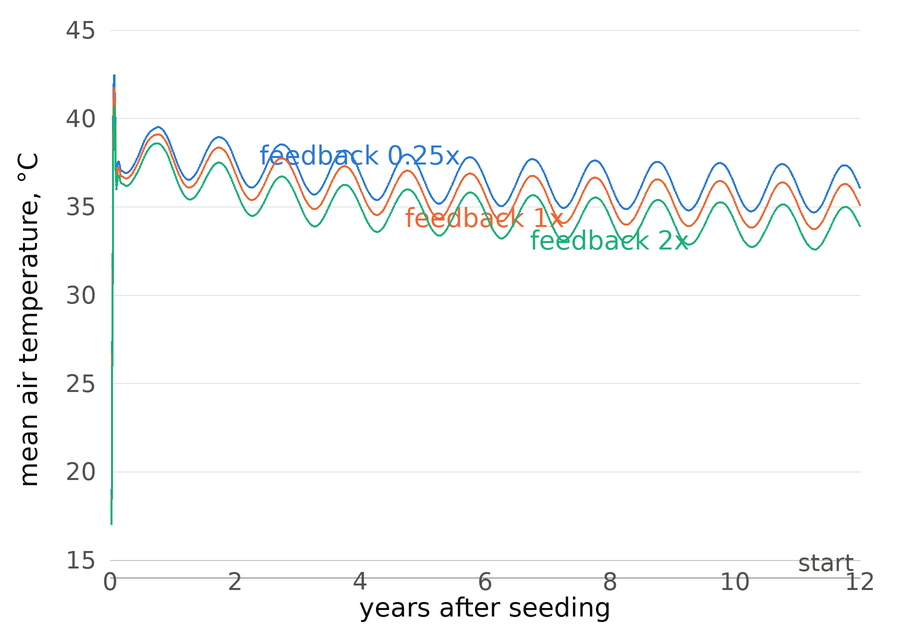
\includegraphics[width=0.49\textwidth]{cool_air.png}
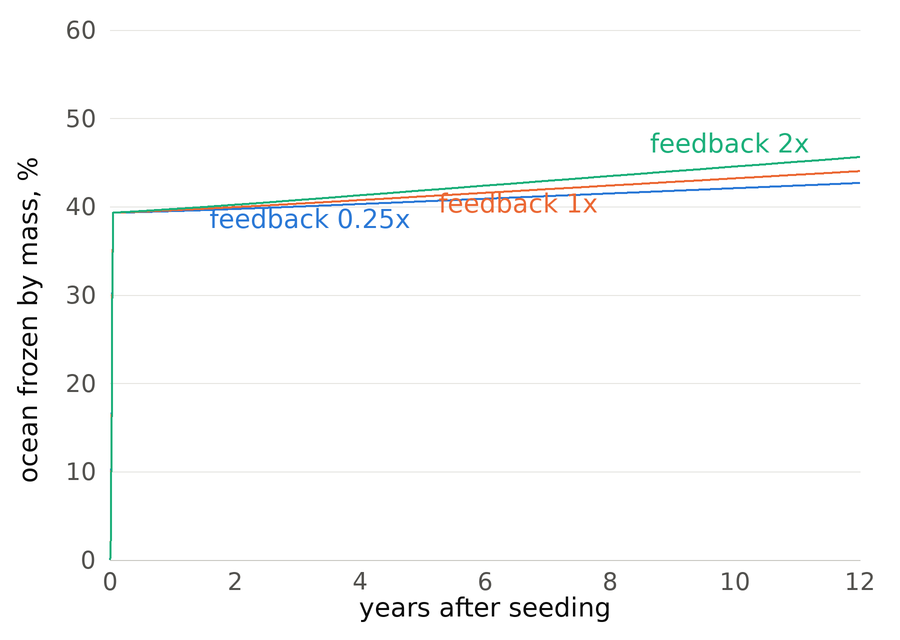
\includegraphics[width=0.49\textwidth]{cool_frozen.png}
\caption{Radiative response scaled by 0.25, 1 and 2. Left: mean air temperature. Right: ocean frozen by mass.}
\label{fig:cool}
\end{figure}

\subsection{Settings with little effect}

Removing the diurnal and seasonal cycle, removing currents and storm seeding, setting a uniform depth, removing snowfall, or changing the convective cap between 1.5 and 5~K changes the twelve-year frozen fraction by at most one percentage point. Uniform depth raises the final air temperature by 2.9~K, probably because there are no shallow shelves to cool and freeze first. Removing snowfall moves the air peak from the first weeks to the first summer and lowers it by 3~K, because the slower front releases its heat over a longer time.

\subsection{Depth}
\label{sec:depth}

Depth affects the solid fraction but not the temperature (Table~\ref{tab:depth}). All columns reach about 40\% solid and 42~\degC\ in the first phase. A column at its melting point stays there while it loses heat, because the heat lost goes into further freezing. Heat loss per unit area is similar for all columns, so shallow columns freeze faster per unit depth. After eight years, columns shallower than 200~m are 69\% solid and 12--14\% are frozen through; columns deeper than 3000~m are 42--43\% solid.

\begin{table}[htbp]
\centering\small
\caption{Solid fraction and temperature by depth (sinking solid). The last column is the share of columns frozen through at 8.2 years.}
\label{tab:depth}
\begin{tabular}{lrrrrrrr}
\toprule
& \multicolumn{2}{c}{60 days} & \multicolumn{2}{c}{3.3 years} & \multicolumn{3}{c}{8.2 years} \\
\cmidrule(lr){2-3}\cmidrule(lr){4-5}\cmidrule(lr){6-8}
Depth & $\phi$ & $T$ (\degC) & $\phi$ & $T$ & $\phi$ & $T$ & frozen \\
\midrule
< 100 m & 0.42 & 41.7 & 0.60 & 38.6 & 0.70 & 35.0 & 14\% \\
100--200 m & 0.41 & 42.0 & 0.58 & 39.2 & 0.69 & 35.7 & 12\% \\
200--500 m & 0.41 & 42.1 & 0.51 & 41.0 & 0.59 & 39.1 & 1.5\% \\
500--1500 m & 0.41 & 42.1 & 0.48 & 41.4 & 0.56 & 39.8 & 0.4\% \\
1500--3000 m & 0.40 & 42.1 & 0.42 & 42.0 & 0.46 & 41.7 & 0 \\
3000--4500 m & 0.40 & 42.2 & 0.41 & 42.1 & 0.43 & 41.9 & 0 \\
> 4500 m & 0.39 & 42.2 & 0.40 & 42.1 & 0.42 & 42.0 & 0 \\
\bottomrule
\end{tabular}
\end{table}

\subsection{Floating solid}
\label{sec:floats}

With a floating solid, the mixed layer freezes to about 30\% of the surface in the first week and then loses heat to the air. The crust covers 50\% of the surface after 1.1 years, 90\% after 4.3 years and 99\% after 5.8 years (Figure~\ref{fig:long}). The deep ocean does not wait for the crust. Brine rejected by the crust makes the water below it denser than the deep water, the column overturns, and the deep water freezes against the crystals: the deep layer is 10\% solid after 30 days, 30\% after one year and 41\% after two, at 41.8~\degC. The ocean is 31\% frozen by mass after one year and 42\% after two, and ends at 43.7\%, the value Eq.~\eqref{eq:stall} gives for deep water at about 2~\degC. Front speed has no effect on these numbers after the first month.

The air peaks at 41~\degC\ on day 19 (2-hour steps), stays above 30~\degC\ for two years, falls below its initial 14~\degC\ after 4.7 years as the crust and the snow-covered land reflect more sunlight, passes 0~\degC\ after 5.6 years, and is $-27$~\degC\ after eight years and $-37$~\degC\ after twelve. After eight years the air is 39--48~K below today's climatology in every latitude band from 60\degree S to the North Pole, and 29~K below it over Antarctica. Rain over land stops once the crust closes, because the ocean no longer evaporates.

Three processes deepen this cooling. Clouds expose the crust: under a dry crust the vapour falls, cloud cover drops from 0.80 after 30 days to 0.28 after eight years, and the white surface shows through more than under today's 0.67; without clouds the run ends at $-16.6$~\degC, 20~K warmer. Snow on land adds reflection: without snowfall the air passes 14~\degC\ after 5.1 years and ends at $-25.5$~\degC. The water-vapour greenhouse amplifies the albedo cooling as it would amplify a warming; without it the crust closes earlier (5.2 years, because the air sheds heat faster while warm) and the run ends at $-29.4$~\degC.

\begin{figure}[htbp]
\centering
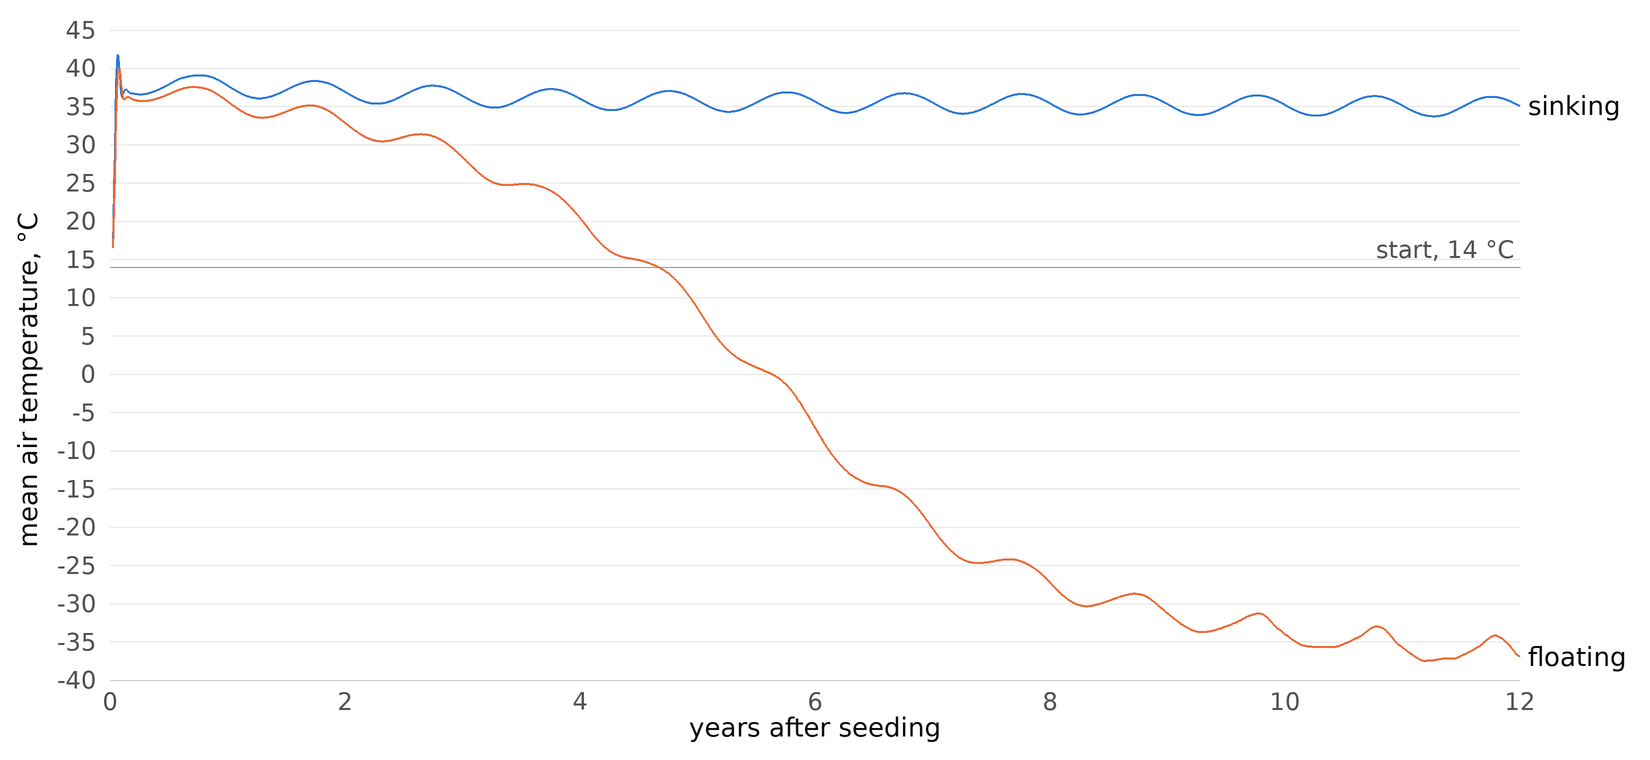
\includegraphics[width=\textwidth]{long_air.png}\\[6pt]
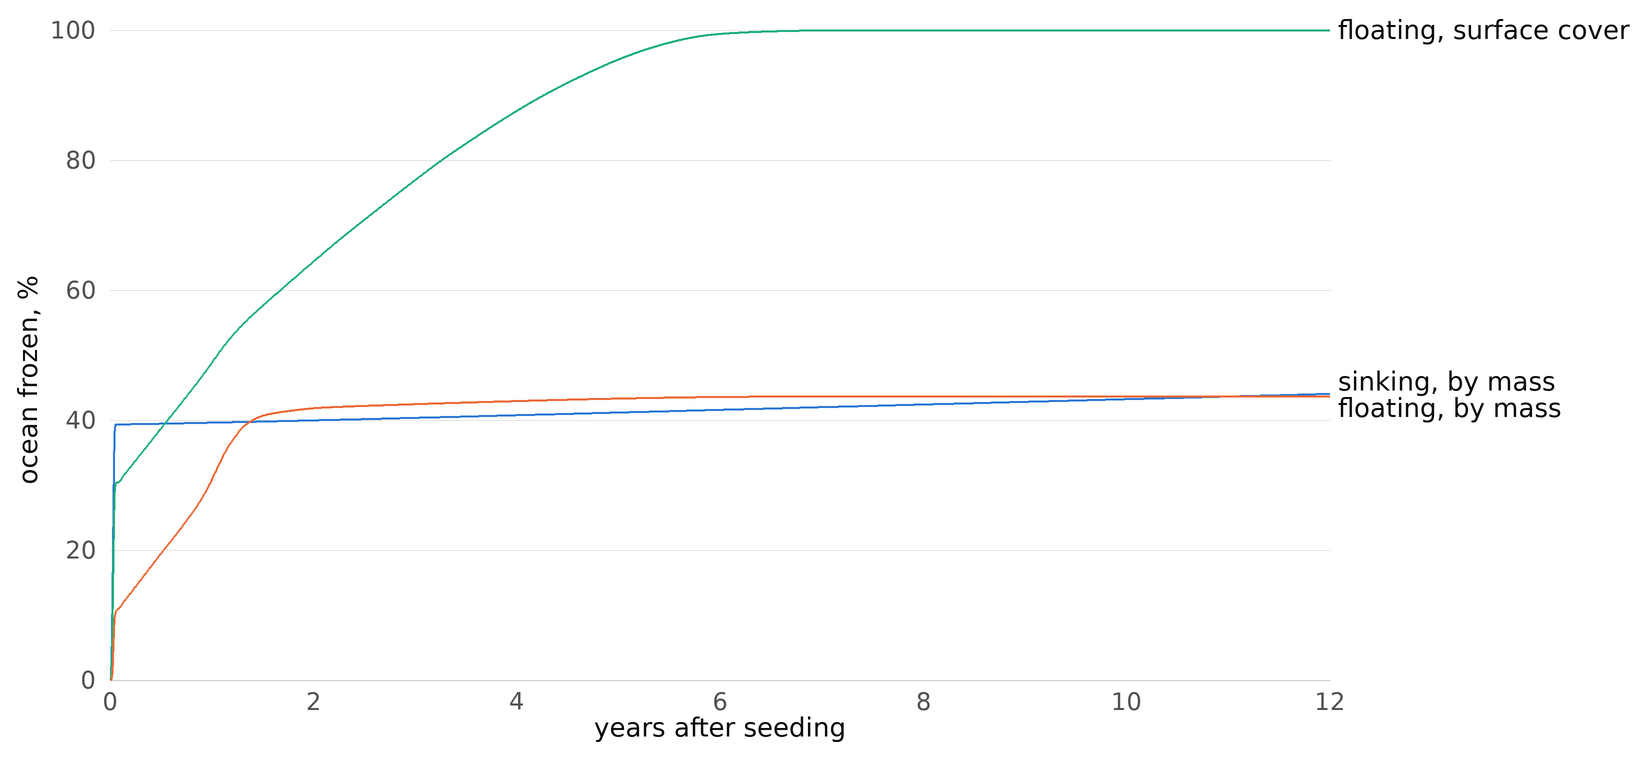
\includegraphics[width=\textwidth]{long_frozen.png}
\caption{Sinking and floating solid over twelve years (48-hour steps). Top: mean air temperature; the yearly oscillation is the seasonal cycle. Bottom: ocean frozen by mass, and surface ice cover for the floating case.}
\label{fig:long}
\end{figure}

\subsection{Leads in the crust}
\label{sec:leads}

The floating results assume a sealed crust. Real sea ice is not sealed: wind and currents keep 1--3\% of the Arctic pack open as leads in winter. We tested how much the snowball depends on the seal with an optional lead share: where the crust covers more than $1-f$ of a column, the missing open share $f$ exposes the deep layer's liquid, at its melting point near 42~\degC\ under a closed crust, to the air at the same bulk rates as an open sea surface. The heat comes out of the deep layer, which then freezes against the crystals; the turbulent part warms the air and the vapour it carries, the longwave part leaves directly. Leads also loft crystals, count as open water for evaporation, and are dark. The energy residual with $f = 3\%$ is the same as without leads (Section~\ref{sec:conv}). The runs in Table~\ref{tab:leads} use a fixed random seed; the sealed run ends 0.3~K colder than the baseline in Table~\ref{tab:scen}.

\begin{table}[htbp]
\centering\small
\caption{Floating solid with a lead share $f$ of the crust kept open (0.5\degree\ grid, 48-hour steps, twelve years, fixed seed). Ocean frozen by mass after twelve years; year in which 99\% of the surface is ice-covered; year in which the air falls below 0~\degC; mean air temperature after eight and twelve years, and after twelve years without clouds.}
\label{tab:leads}
\begin{tabular}{lrrrrrr}
\toprule
$f$ & Frozen (\%) & 99\% covered & Air $<0$~\degC & Air 8 yr & Air 12 yr & No clouds 12 yr \\
\midrule
sealed & 43.7 & 5.77 & 5.6 & $-27.4$ & $-37.4$ & $-16.6$ \\
0.1\% & 43.7 & 5.78 & 5.7 & $-25.4$ & $-34.5$ & -- \\
0.3\% & 43.9 & 5.80 & 5.8 & $-21.9$ & $-29.6$ & -- \\
0.5\% & 44.0 & 5.83 & 5.9 & $-18.9$ & $-25.8$ & -- \\
1\% & 44.3 & 5.88 & 6.0 & $-12.9$ & $-18.3$ & $-9.9$ \\
3\% & 45.0 & 6.09 & 8.1 & 1.0 & $-2.0$ & $-0.5$ \\
5\% & 45.4 & 6.28 & -- & 8.4 & 6.3 & 5.7 \\
\bottomrule
\end{tabular}
\end{table}

The snowball is sensitive to the seal from the first tenth of a percent. Each 0.1 percentage point of leads up to 1\% warms the air after twelve years by 1.5--3~K; 1\% leaves it at $-18$~\degC, 19~K warmer than sealed, and 5\% keeps it above 0~\degC. The first year and the ocean's end state hardly change: leads act only where the crust is nearly closed, and the extra heat they draw freezes the deep ocean a little further, to 45\% at 5\%. The cause is the heat stored under the crust. Through a lead, water near 42~\degC\ meets air at $-30$~\degC\ or colder and loses about 7~kW/m$^2$, so 1\% of leads sheds about 65~W/m$^2$ over the crust, of the same order as the 102~W/m$^2$ by which a white ocean cools the planet.

Leads act both directly and through the clouds. Without clouds, leads warm the air after twelve years by 7, 16 and 22~K at 1, 3 and 5\%; with clouds by 19, 35 and 44~K. The vapour from the leads keeps the clouds that would otherwise thin over a dry crust and expose it. The cloud cooling of Section~\ref{sec:floats}, 21~K for the sealed crust, falls to 8~K at 1\% leads and to 1.5~K at 3\%. The two effects are therefore not independent: the clouds deepen the snowball only because the crust is sealed.

The lead share is not known, and the test overstates it. A real lead at an air-water difference of 70--80~K skins over within minutes and then loses heat by conduction through the new ice. With the conductivity of ordinary ice, 2~W/m/K, assumed for ice-nine, the new ice is about 0.3~m thick after a day and 0.9~m after ten days. A lead opened at rate $r$ and refreezing for a time $\tau$ is then equivalent to an open share of about $r\,\rho L\,d(\tau)/F_\mathrm{open}$; for Arctic winter opening of 0.3--1\% of the area per day and $\tau$ of 10--30 days this is 0.15--0.9\%. Whether a crust tens of metres thick opens leads at all is open; a thick crust may behave more like an ice shelf than like pack ice, and thermal contraction as the crust cools (about 0.4\% for 80~K with the expansion coefficient of ordinary ice) opens cracks once, and mostly in its cold upper part. Expansion on freezing closes leads rather than opening them. Within 0.15--0.9\% the floating case ends 4--18~K warmer than sealed, between about $-33$ and $-20$~\degC\ after twelve years, still far below today's temperature. The crust still closes, and the deep ocean still freezes to its limit.

\subsection{Life in the brine}
\label{sec:life}

The brine channels of a floating crust are liquid, lit and salty. Algae live in the brine of ordinary sea ice today, and halotolerant cyanobacteria and \emph{Dunaliella salina} grow in near-saturated brine above 40~\degC. As an option, a bloom grows in crust brine between $-15$ and 45~\degC\ in daylight, and a full bloom removes 13\% of the crust's extra reflection, the albedo loss measured for red snow algae on Arctic glaciers (Lutz et al.\ 2016). The upper temperature limit is an estimate. The bloom delays the cooling: the air passes 14~\degC\ after 4.9 years instead of 4.7, and the crust closes after 6.0 years instead of 5.8. The end state is unchanged ($-37.0$~\degC). The bloom's growth rate and its survival as the crust cools are not constrained; this run shows only that the effect is small.

\subsection{Snowfall on land}
\label{sec:snow}

Sea spray from the slush carries crystals into the air, and the wind spreads them over the continents within days. One crystal freezes a raindrop, and frozen drops freeze the ones they meet, so rain that forms in air carrying crystals falls as ice-nine. The model's threshold, $10^{-4}$ of the crystal concentration over seeded water, corresponds to 1--10 crystals per litre for sea-spray concentrations of $10^7$--$10^8$ per m$^3$, comparable to the ice-nucleus concentrations that glaciate ordinary cold clouds.

With 2-hour steps land is 59\% white after 7 days and 93\% after 10 (Figure~\ref{fig:snow}). The evaporating slush ocean raises rain over land to 6.4 times today's on day 10, 3 times after 30 days, 1.9 times after a year and 1.3 times after eight years, so 2~cm of water equivalent, enough to hide the ground, accumulates within days almost everywhere.

The snow survives because of the two melting points. Land snow is fresh ice-nine and melts at 45.8~\degC. The sea slush melts at 43.6~\degC\ or lower as brine concentrates, and moist convection keeps the air within a few kelvin of the sea surface. The air over a slush ocean therefore stays mostly below the snow's melting point. The exception is continental summer: in the first year snow cover falls to 86\% (91\% with 2-hour steps) as the air over the northern mid-latitude continents rises above 45.8~\degC, and recovers in autumn. From the second summer on the land stays white. With a 5~K convective cap the first-summer dip goes to 84\%, with 1.5~K to 88\%.

Snow on land cools the planet but does not change the ocean's twelve-year result: 44\% with snowfall, 43\% without. In the sinking case it changes the air after twelve years by less than 0.5~K; in the floating case by 12~K.

Ice-nine snow does not melt off or run into rivers, so it holds water on land. In the sinking baseline the land holds the equivalent of 0.43~m of the global ocean after one year, 1.7~m after four and 3.2~m after eight years. In the floating case accumulation slows as rain fails and stops when the crust closes, at about 2.0~m. The model does not remove this water from the ocean; 3.2~m is less than 0.1\% of the ocean's volume.

\begin{figure}[htbp]
\centering
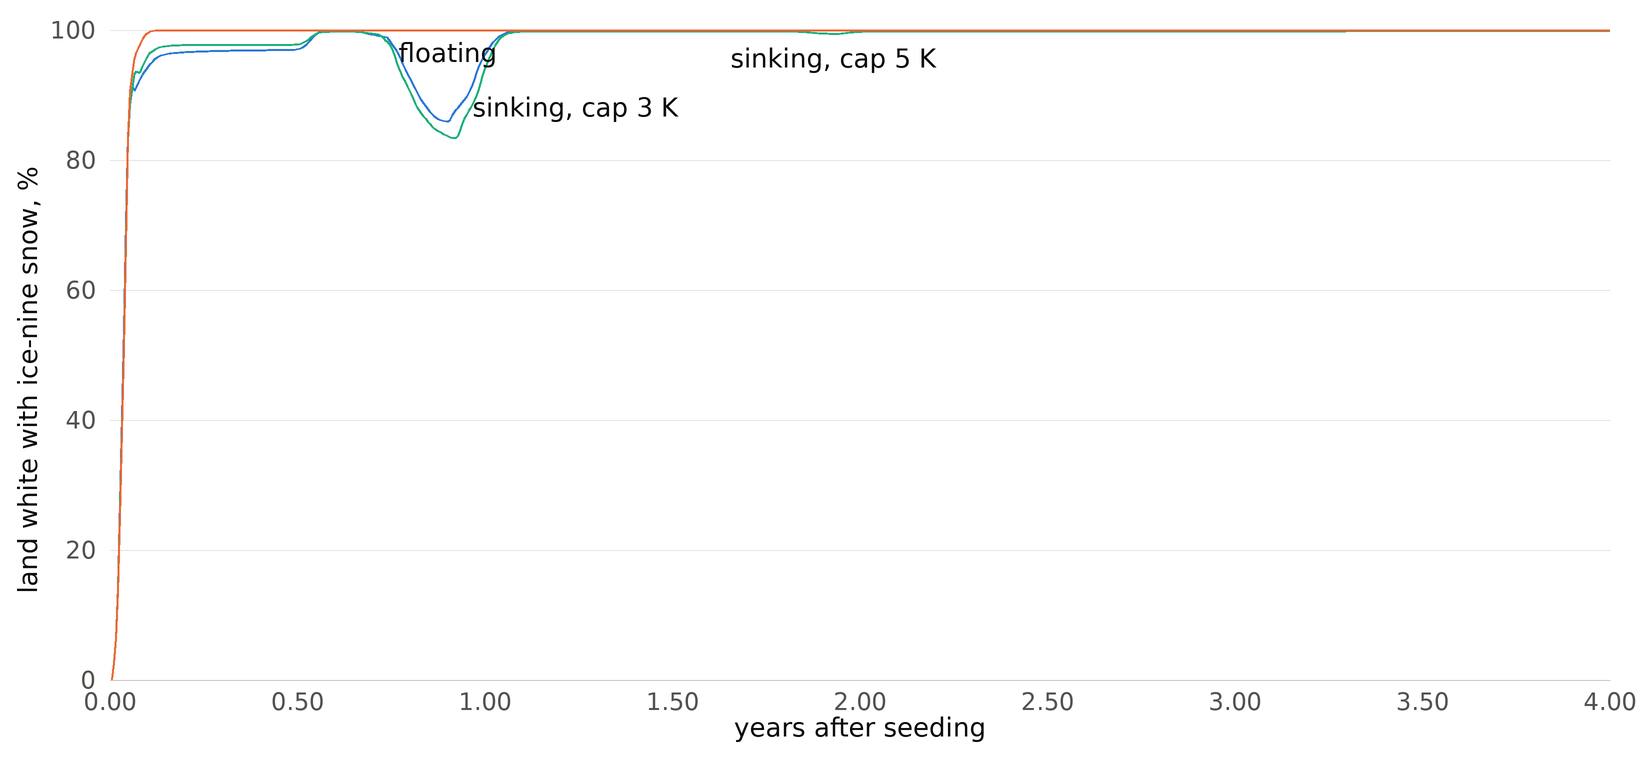
\includegraphics[width=\textwidth]{snow.png}
\caption{Land covered by ice-nine snow in the first four years (48-hour steps). The dips are northern summers.}
\label{fig:snow}
\end{figure}

\subsection{How robust the snow is}
\label{sec:snowsens}

The snow result rests on three crystal parameters with no observational basis (lofting time, washout time, freezing threshold) and on the rain over land. We varied them in a factorial sweep of 54 one-year runs (1\degree\ grid, 48-hour steps, sinking case): lofting $\times$0.01 to 1, threshold $\times$1 to 100, washout $\times$1 to 3, and rain over land as today plus the extra vapour, today only, or half today plus a quarter of the extra. Table~\ref{tab:snowsens} shows selected rows.

\begin{table}[htbp]
\centering\small
\caption{Land white with ice-nine snow (\%) after 30 days, at the first-summer minimum and after one year, as all land / deserts (today under 250~mm/yr) / interiors (over about 1000~km from the sea). 1\degree\ grid, 48-hour steps, sinking solid.}
\label{tab:snowsens}
\begin{tabular}{lccc}
\toprule
Setting & 30 days & first summer & 1 year \\
\midrule
Baseline & 88/85/82 & 80/65/64 & 94/86/94 \\
Lofting $\times$0.01 & 73/66/57 & 73/55/52 & 84/61/71 \\
Threshold $\times$100 & 65/58/45 & 66/47/42 & 78/50/61 \\
Washout $\times$3 & 56/42/38 & 60/36/36 & 70/37/48 \\
No extra rain & 59/11/51 & 47/21/27 & 64/23/48 \\
Half rain, quarter extra & 70/58/66 & 48/26/28 & 67/31/57 \\
Washout $\times$3, threshold $\times$10 & 38/20/23 & 53/29/29 & 61/30/36 \\
All three crystal factors pessimistic & 0/0/0 & 11/8/2 & 16/12/4 \\
\bottomrule
\end{tabular}
\end{table}

Of the 54 combinations, 5 keep more than 80\% of land white after one year and 29 keep more than 50\%. Washout and the extra rain matter most; deserts and continental interiors are the least robust. We therefore separate three levels of confidence:
\begin{itemize}
\item \textbf{High:} rain falling through air that carries crystals freezes and lands as ice-nine, and that snow survives wherever the air stays below 45.8~\degC. This follows from the melting points.
\item \textbf{Medium:} ice-nine snow covers a large part of the land in the first year, most of it near coasts and in wet regions. Most of the sweep supports this.
\item \textbf{Low:} near-complete cover within weeks, including deserts and interiors. Only the baseline and the most favourable settings give it.
\end{itemize}
The ocean results do not depend on the snow: removing snowfall changes the twelve-year frozen fraction by one percentage point in both cases. Rain seeding of the ocean depends on the same parameters and sets only how fast the first phase ends.

\subsection{Unfreezable water}

Water above its own melting point cannot take the lattice. In these runs at most 0.1\% of the ocean is ever in that state, and at most 0.2\% of the shelf seas melt back after freezing. Two effects produce it: tropical water reached late after the air above it has warmed, and shallow shelves next to continents whose summer air is above the melting point. Both are visible on the maps as red cells along some coasts.

\subsection{Maps}

Figure~\ref{fig:maps} shows both cases. After 24 days the land is white and the sea is seeded almost everywhere, from the sky as much as from the front. With a sinking solid the surface remains open slush at about 42~\degC; after eight years only the shelves and polar seas are solid through. With a floating solid the map after eight years is uniformly white, ocean and land, so the bottom row shows the solid fraction of the whole column instead.

\begin{figure}[htbp]
\centering
\begin{tabular}{@{}cc@{}}
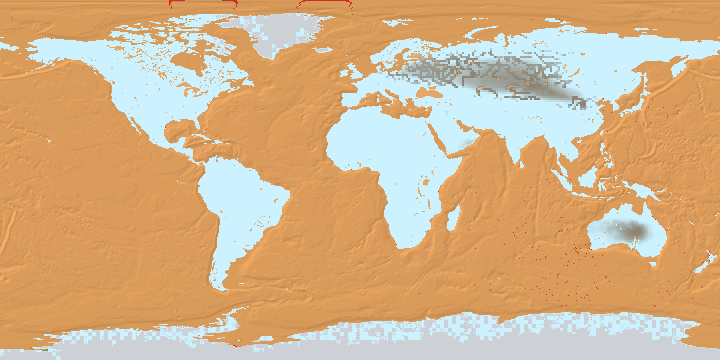
\includegraphics[width=0.485\textwidth]{map_sinks_24d.png} &
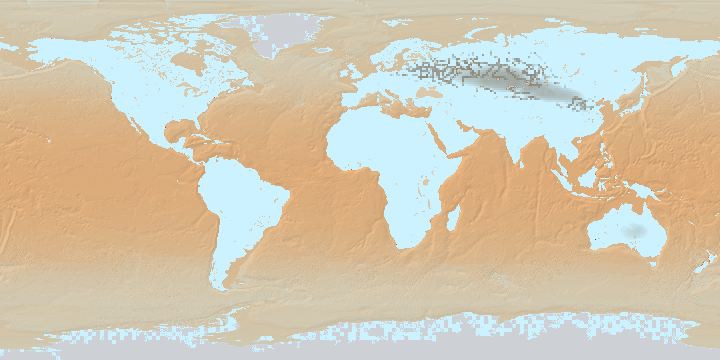
\includegraphics[width=0.485\textwidth]{map_floats_24d.png} \\
\small sinking, day 24 & \small floating, day 24 \\[4pt]
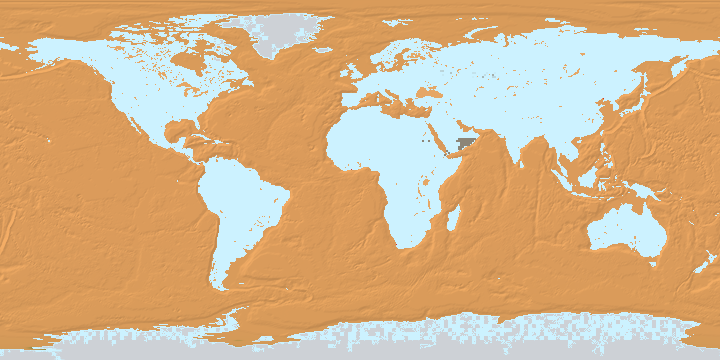
\includegraphics[width=0.485\textwidth]{map_sinks_80d.png} &
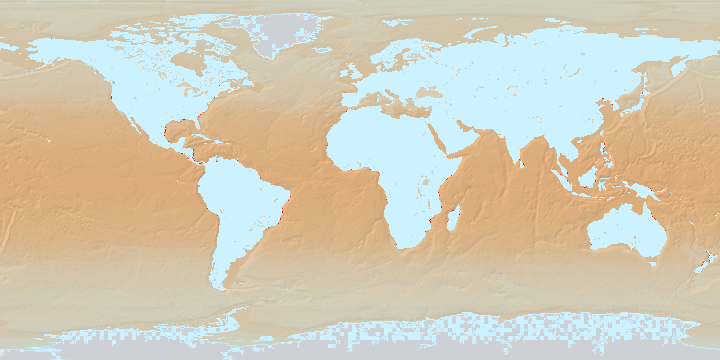
\includegraphics[width=0.485\textwidth]{map_floats_80d.png} \\
\small sinking, day 80 & \small floating, day 80 \\[4pt]
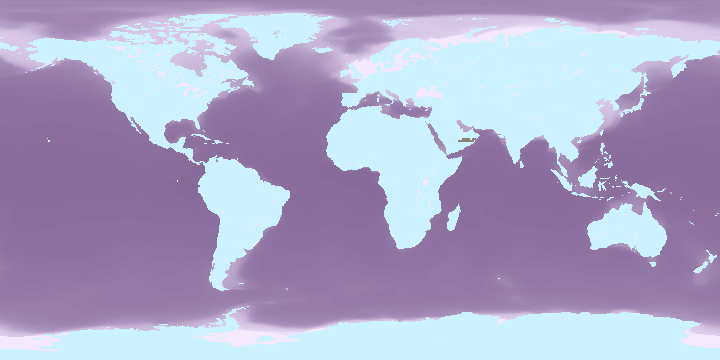
\includegraphics[width=0.485\textwidth]{overlay_sinks_8y.png} &
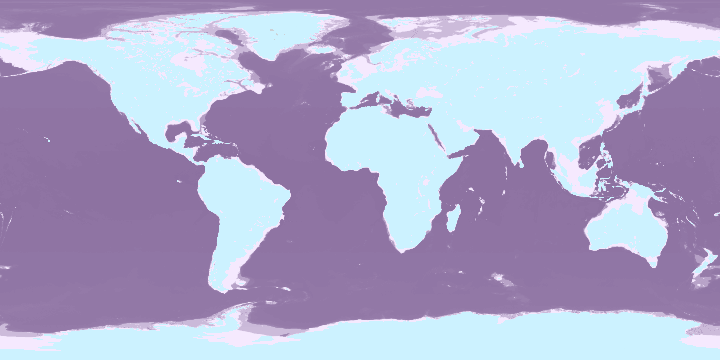
\includegraphics[width=0.485\textwidth]{overlay_floats_8y.png} \\
\small sinking, year 8, solid fraction & \small floating, year 8, solid fraction \\
\end{tabular}
\caption{Top and middle: surface state. Water is coloured by temperature (navy cold, amber near the melting point, red above it); blue-white is ice-nine at the surface or as snow on land; grey is ordinary ice. Bottom: solid fraction of the whole column (dark purple little, light fully frozen); land shows its snow cover.}
\label{fig:maps}
\end{figure}

\section{Air temperature}
\label{sec:air}

In an hourly run on a 0.25\degree\ grid the mean air temperature rises from 14~\degC\ to 34~\degC\ after 10 days and peaks at 43~\degC\ on day 16, then falls back to 35--36~\degC\ by day 30 (Figure~\ref{fig:air}). The overshoot follows the burst of heat released by rain-seeded freezing in the first week; the air then sheds the excess to space and settles over the sea, which sits at its melting point. In the sinking case the air then stays near 36--38~\degC\ for two years and declines slowly after that, to 35~\degC\ after twelve.

The warming is not uniform. The sea surface warms by its distance from the melting point: 40~K at 60--90\degree N and 38~K at 60--90\degree S, 28~K at 30--60\degree, and 17~K in the tropics. The air follows the sea: after one year it is 39~K above its climatology at 60--90\degree N and 17~K in the tropics. Polar amplification here comes from the cold start of polar water, not from ice or snow feedbacks.

The diurnal cycle produces a daily oscillation of about 0.02~K in the global mean air temperature during the first month (Figure~\ref{fig:wobble}). The seasonal cycle produces a yearly oscillation of about 3~K (Figure~\ref{fig:long}).

\begin{figure}[htbp]
\centering
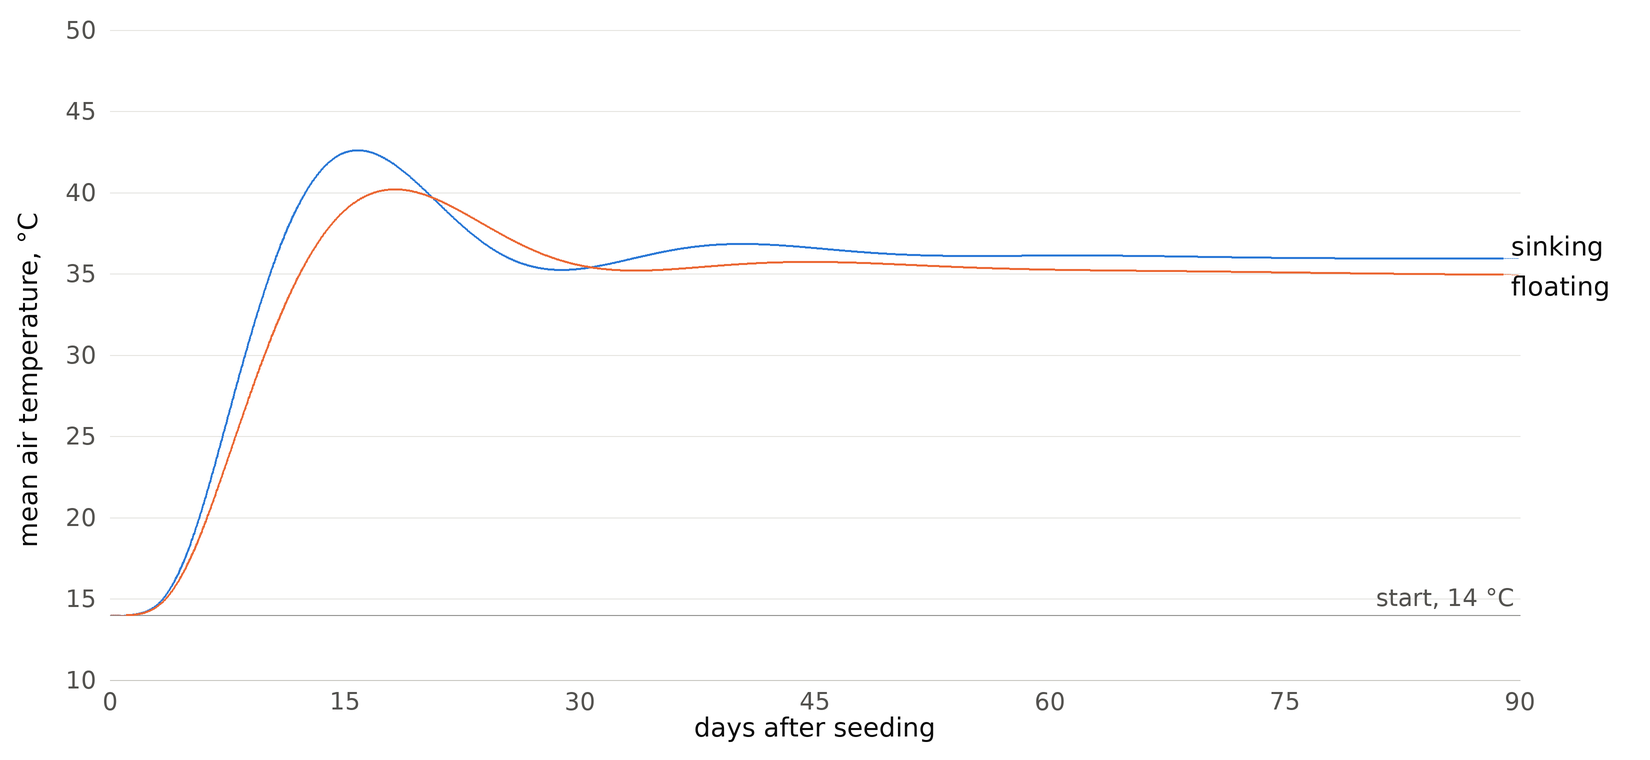
\includegraphics[width=\textwidth]{air.png}
\caption{Mean air temperature in the first 90 days (0.25\degree\ grid, hourly).}
\label{fig:air}
\end{figure}

\begin{figure}[htbp]
\centering
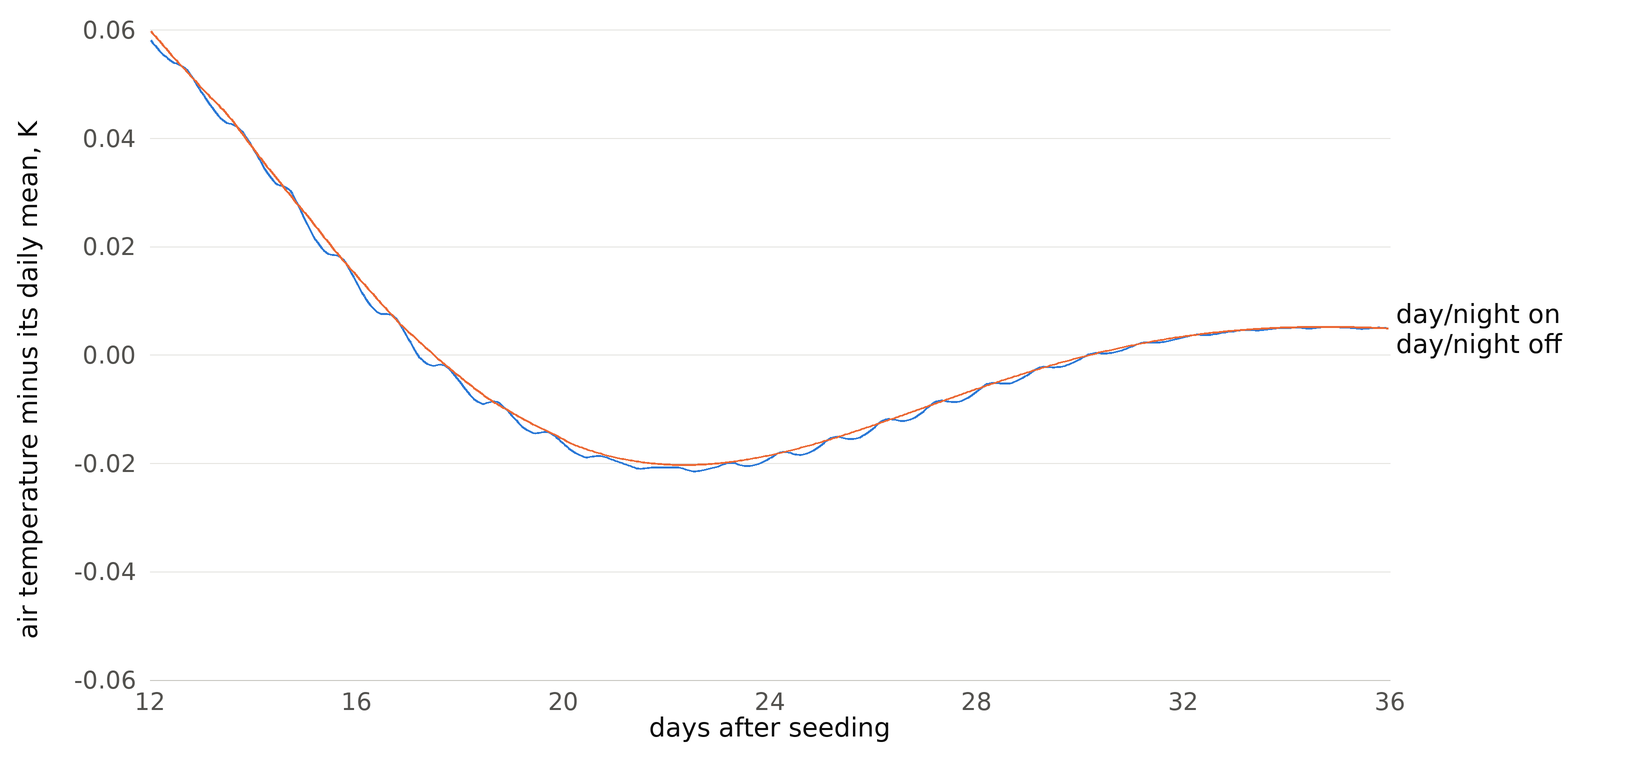
\includegraphics[width=\textwidth]{wobble.png}
\caption{Air temperature minus its daily mean, with and without the diurnal cycle (sinking solid, 0.25\degree, hourly).}
\label{fig:wobble}
\end{figure}

\section{Conservation and convergence}
\label{sec:conv}

\paragraph{Energy.} The model keeps a ledger of heat leaving the system (to space from the air and from the sea surface) and compares it with the change in stored heat: sensible heat of the ocean, deep layer, inland water, ice sheets and air, latent heat held in solid ice-nine and in snow, and the latent heat of extra vapour in the air. After one and three years the residual is at most 0.03\% of the latent heat released, in both cases.

\paragraph{Mass.} Salt is conserved to a relative $6\times10^{-9}$ in the floating case, where brine moves between layers. Water moved to land as snow is counted but, as stated above, not removed from the ocean.

\paragraph{Convergence.} Table~\ref{tab:conv} repeats both baselines on four grids (1\degree\ to 0.125\degree), three time steps (48, 12 and 2 hours) and three random seeds. The 0.125\degree\ runs stop after one year.

\begin{table}[htbp]
\centering\small
\caption{Convergence. Day on which 90\% of land is white; day on which 38\% of the ocean is frozen (sinking only); ocean frozen by mass (\%) after 30 days, 1 and 3 years; mean air temperature (\degC, mean over the preceding two days) after 1 and 3 years.}
\label{tab:conv}
\setlength{\tabcolsep}{4pt}
\begin{tabular}{lrrrrrrr}
\toprule
& \multicolumn{2}{c}{day} & \multicolumn{3}{c}{frozen (\%)} & \multicolumn{2}{c}{air (\degC)} \\
\cmidrule(lr){2-3}\cmidrule(lr){4-6}\cmidrule(lr){7-8}
Run & white & 38\% & 30 d & 1 yr & 3 yr & 1 yr & 3 yr \\
\midrule
\multicolumn{8}{l}{\emph{Sinking}} \\
1\degree, 48 h & 44 & 20 & 39.3 & 39.5 & 40.2 & 38.2 & 36.6 \\
0.5\degree, 48 h & 22 & 20 & 39.4 & 39.6 & 40.4 & 37.8 & 36.5 \\
0.25\degree, 48 h & 20 & 18 & 39.3 & 39.7 & 40.4 & 37.4 & 36.3 \\
0.125\degree, 48 h & 20 & 18 & 39.3 & 39.7 & -- & 37.1 & -- \\
0.5\degree, 12 h & 12 & 11 & 39.4 & 39.6 & 40.4 & 37.5 & 36.2 \\
0.5\degree, 2 h & 10 & 7 & 39.4 & 39.6 & 40.4 & 37.4 & 36.1 \\
0.5\degree, 48 h, seed 2 & 22 & 20 & 39.4 & 39.6 & 40.4 & 37.8 & 36.5 \\
0.5\degree, 48 h, seed 3 & 22 & 20 & 39.3 & 39.6 & 40.4 & 37.8 & 36.5 \\
\multicolumn{8}{l}{\emph{Floating}} \\
1\degree, 48 h & 24 & -- & 10.8 & 28.8 & 42.2 & 36.4 & 29.9 \\
0.5\degree, 48 h & 20 & -- & 10.9 & 30.7 & 42.5 & 35.7 & 28.4 \\
0.25\degree, 48 h & 20 & -- & 10.9 & 31.7 & 42.5 & 35.1 & 27.4 \\
0.125\degree, 48 h & 20 & -- & 10.9 & 32.8 & -- & 34.6 & -- \\
0.5\degree, 12 h & 13 & -- & 10.7 & 29.4 & 42.5 & 35.3 & 26.5 \\
0.5\degree, 2 h & 10 & -- & 10.3 & 28.4 & 42.4 & 35.2 & 24.6 \\
0.5\degree, 48 h, seed 2 & 20 & -- & 10.9 & 30.7 & 42.5 & 35.7 & 28.4 \\
0.5\degree, 48 h, seed 3 & 20 & -- & 10.9 & 30.7 & 42.5 & 35.7 & 28.4 \\
\bottomrule
\end{tabular}
\end{table}

The sinking case has converged from day 30 on: the frozen fraction varies by at most 0.4 percentage points across grids, steps and seeds, and the air after one year by about 1~K. The floating case has converged in its end state (42.2--42.5\% after three years) but not in its timing. Finer grids freeze faster and shorter steps slower: the frozen fraction after one year ranges from 28\% to 33\%, and the air after three years from 25 to 30~\degC. The floating timeline in Figure~\ref{fig:timeline} is therefore uncertain by several months, possibly up to a year; the order of events is not.

The first weeks depend on the time step. With 48-hour steps the sinking stall comes on day 18--20, with 12-hour steps on day 11, with 2-hour steps on day 7 and in the hourly 0.25\degree\ run on day 6. The cause is in the model: the water cycle and snowfall are updated once per step, so each round of seeded sea, lofted crystals, rain and new seed waits a full step. This round is the fastest process in the model, and the 2-hour and hourly runs are close to each other, so we take day 6--7 as the model's answer. All values in Table~\ref{tab:scen} from day 30 on are unaffected.

\section{Limitations}

The atmosphere is a single layer with prescribed feedbacks, not a radiative transfer or circulation model. The water-vapour greenhouse is one curve fitted between today's feedback and the runaway threshold. The reflection and trapping of the extra cloud in a much wetter world are not modelled; their net sign is unknown, and they could change the air temperature by several kelvin in either direction. The floating snowball depends strongly on how cloud cover responds to a dry crust, which is a prescribed curve. It depends as strongly on the crust being sealed: an open-water equivalent of 1\% of leads makes it 19~K warmer, and the lead share is not known (Section~\ref{sec:leads}). The air's warming is limited to 3~K above the sea's by a prescribed convective cap. Rain over land keeps today's spatial pattern plus the extra vapour carried by the wind; changes in circulation are not modelled. The three crystal parameters are estimates and the snow cover depends on them (Section~\ref{sec:snowsens}). The water held on land as snow is not removed from the ocean.

Other limitations: the front speed, storm seeding rate and current amplitudes are prescribed; there is no ocean circulation below the surface and no vertical structure beyond two layers; the overturn velocity is a typical value, not derived; salt precipitation is not modelled; in the floating case the surface exchange uses the mixed-layer temperature rather than a separate crust-surface temperature; the 48-hour scenario runs delay the first weeks (Section~\ref{sec:conv}).

Freezing the whole ocean releases about $5\times10^{26}$~J. In the second phase the sinking case sheds this at a rate that would take about 140 years to freeze the remaining 56\% of the ocean.

\section{Changes from the earlier version of this paper}

An earlier version of 18 October 2026 reported a stall at 35\% after a month and a floating end state of $-16$~\degC. Since then the model has changed as follows. Latent heat now follows Kirchhoff's law for a solid with half the heat capacity of water, and heat flows use the column's actual heat capacity; the energy residual fell from 2--3.5\% to under 0.03\%. Rain carrying crystals now seeds the open sea, not only lakes and rivers, and storm seeding is used only when snowfall is off, so the sea is not seeded twice. The latent heat of extra evaporation travels with the vapour and is released where it rains, and evaporation comes only from the unfrozen surface. Brine overturn is a rate (0.02~m/s) instead of a full mix once per step, which had made the floating case depend on the step. The convective cap spreads its excess over the atmosphere instead of discarding it. The combined effect: the stall is larger (39\%) and comes within a week, the floating crust closes later (5.8 instead of 5.7 years), and the floating case ends 21~K colder. The individual contributions to the colder end state were not separated. The model also has an optional lead share in the floating crust (Section~\ref{sec:leads}); all other results use a sealed crust, as before. Finally, today's rain over land now comes from the GPCC climatology instead of WorldClim~2.1, whose terms do not allow the derived grid to be redistributed with the model; over land the two agree to within 1\% on average, and the results changed by at most a few tenths of a unit.

\section{Conclusions}
\label{sec:conc}

\begin{enumerate}
\item With latent heat included, ice-nine does not freeze the ocean quickly. About 39\% of the ocean freezes within a week; the fraction is set by the latent heat, 23--46\% for 669--334~kJ/kg.
\item The week is set by rain. Crystals in the air freeze the rain, and that rain seeds the sea, lakes and rivers everywhere it falls. Without it the front needs about two months.
\item Further freezing is limited by radiation to space and proceeds at about 0.4 percentage points per year in the sinking case. Complete freezing would take more than a century.
\item Within two weeks, ice-nine snow covers most land. It persists because fresh ice-nine melts above the brine-depressed slush that sets the air temperature, and it holds metres of ocean-equivalent water on land within a decade. Its extent depends on crystal parameters that are not known.
\item Whether ice-nine sinks or floats determines the end state. A sinking solid leaves an open slush ocean at about 42~\degC\ under air near 35~\degC\ for at least a decade, with shelves freezing first. A floating solid closes a crust after about six years, freezes the deep ocean to its limit within two years through brine-driven overturn, and cools the planet below today's temperature after five years and to $-37$~\degC\ after twelve. Clouds account for about 20~K of that cooling, but only under a sealed crust: leads of 0.15--0.9\% of the crust, a plausible range, leave the air at about $-33$ to $-20$~\degC.
\item Only the floating case resembles the outcome described in the novel, and it takes years rather than minutes. Known high-pressure ice phases are denser than water, which favours the sinking case.
\end{enumerate}

\end{document}
